% Paper I (ICML format). Build: pdflatex twomoment; bibtex twomoment; pdflatex x2
\documentclass{article}
\usepackage{microtype}
\usepackage{graphicx}
\usepackage{booktabs}
\usepackage{hyperref}
\newcommand{\theHalgorithm}{\arabic{algorithm}}
\usepackage{icml2026}
\usepackage{amsmath,amssymb,mathtools,amsthm}
\usepackage[capitalize,noabbrev]{cleveref}
\theoremstyle{plain}
\newtheorem{theorem}{Theorem}
\newtheorem{proposition}[theorem]{Proposition}
\newtheorem{lemma}[theorem]{Lemma}
\newtheorem{corollary}[theorem]{Corollary}
\theoremstyle{definition}
\newtheorem{definition}[theorem]{Definition}
\newtheorem{assumption}{Assumption}
\renewcommand{\theassumption}{\Alph{assumption}}
\theoremstyle{remark}
\newtheorem{remark}[theorem]{Remark}
% full statements in the appendix carry the number of the main-text statement
\newtheorem*{fullstmt}{\fullstmtname}
\newcommand{\fullstmtname}{}
\newenvironment{full}[2]{\renewcommand{\fullstmtname}{#1~\ref{#2} (full statement)}\begin{fullstmt}}{\end{fullstmt}}
% Shared math macros (master document and both papers). No theorem environments here.
\providecommand{\R}{\mathbb{R}}
\providecommand{\Z}{\mathbb{Z}}
\providecommand{\E}{\mathbb{E}}
\providecommand{\Prob}{\mathbb{P}}
\providecommand{\nnuc}[1]{\|#1\|_{*}}
\providecommand{\nF}[1]{\|#1\|_{F}}
\providecommand{\inner}[2]{\langle #1, #2\rangle}
\providecommand{\tr}{\operatorname{tr}}
\providecommand{\polar}{\operatorname{polar}}
\providecommand{\Med}{\operatorname{Med}}
\providecommand{\dist}{\operatorname{dist}}
\providecommand{\vol}{\operatorname{vol}}
\providecommand{\rank}{\operatorname{rank}}
\providecommand{\Cov}{\operatorname{Cov}}
\providecommand{\He}{\mathrm{He}}
\providecommand{\cA}{\mathsf{A}}
\providecommand{\cB}{\mathsf{B}}
\providecommand{\ones}{\mathbf{1}}
\providecommand{\st}{\dagger}
\providecommand{\ew}{\varepsilon_w}
\providecommand{\Lw}{L_w}
\providecommand{\SO}{\mathrm{SO}}
\providecommand{\Id}{\mathrm{Id}}
\providecommand{\gs}{g_\ast}
\providecommand{\beff}{b_{\mathrm{eff}}}
\providecommand{\cK}{\mathcal{K}}
\providecommand{\cL}{\mathcal{L}}
\providecommand{\Le}{L_\varepsilon}
\providecommand{\psie}{p}
\providecommand{\argmin}{\operatorname*{arg\,min}}

% Shared statements (bodies only). Each document wraps them in its own theorem environments and labels.
% ---------------------------------------------------------------------------------------------
% Definitions and assumptions
% ---------------------------------------------------------------------------------------------
\newcommand{\StmtClass}{%
Fix constants $0<\lambda\le\Lambda$, $C_\ast\ge1$, $c_\ast\in(0,1]$. For $\varepsilon\in(0,1]$, a random vector $X$ in $E$
belongs to the class $\mathcal X(\varepsilon)$ if there are a covariance $\Sigma$ with
$\lambda\,\Id\preceq\Sigma\preceq\Lambda\,\Id$, a symmetric $3$-tensor $\cK$ with $|\cK|\le C_\ast\varepsilon$, and an even
polynomial $\widehat r$ of degree at most $6$ with $\widehat r(0)=0$ and coefficients bounded by $C_\ast\varepsilon^2$,
such that, with the \emph{comparison transform}
$\widehat\psie(t)=e^{-\inner t{\Sigma t}/2}\big(1+\tfrac16\cK[(it)^{\otimes3}]+\widehat r(t)\big)$ and
$\chi_X(t)=\E e^{i\inner tX}$, $a=c_\ast/\varepsilon$:
\begin{itemize}
\item[\textup{(E1)}] $\int_{t_0+[-a,a]^N}|\chi_X(t)|\,dt\le C_\ast$ for every $t_0\in E$;
\item[\textup{(E2)}] $\int_{[-a,a]^N}|\chi_X(t)-\widehat\psie(t)|\,dt\le C_\ast\varepsilon^3$;
\item[\textup{(E3)}] $\Prob(|X|>u)\le C_\ast e^{-u^2/C_\ast}$ for all $u\ge0$.
\end{itemize}
The \emph{comparison density} is the signed density $\psie$ with $\int e^{i\inner ty}\psie(y)dy=\widehat\psie(t)$; explicitly
$\psie=\varphi_\Sigma\,(1+\frac16\inner{\cK}{\He_3^\Sigma}+r)$ with $r$ an even polynomial. Constants denoted $C,c$ in
statements about $\mathcal X(\varepsilon)$ depend only on $N$, $\nu$, $\lambda,\Lambda,C_\ast,c_\ast$.}

\newcommand{\StmtAssB}{%
$\zeta,\zeta_1,\zeta_2,\dots$ are i.i.d.\ in $E$ with $|\zeta|\le M$ almost surely, $\E\zeta=0$, and covariance
$\Sigma\succeq\lambda\,\Id$, $\lambda>0$; $K_3=\E\zeta^{\otimes3}$. A \emph{weight sequence} is $w=(w_k)_{k\ge1}$ with
$w_k\ge0$, $\sum_kw_k=1$; we set
\[
\rho_p=\sum_kw_k^p,\quad\ \xi_w=\sum_kw_k\zeta_k,\quad\ X_w=\rho_2^{-1/2}\xi_w,\quad\
\ew=\frac{\max_kw_k}{\sqrt{\rho_2}},\quad\ \Lw=\log(e/\ew).
\]
No condition is imposed on the characteristic function of $\zeta$.}

\newcommand{\StmtAssR}{%
There is a closed cone $V\subset E$ such that $o\in C^\infty(E\setminus V)$,
$|D^ko(y)|\le C_k\dist(y,V)^{-k}$ for all $k\ge0$, and
$\vol\{y\in B(0,1):\dist(y,V)\le r\}\le C_Vr^{c}$ for $r\le1$.}

\newcommand{\StmtAssL}{%
$N\ge3$, and there are $\kappa\in(0,1]$ with $2+\kappa<N$ and a constant $C$ such that the Fourier transform of the
finite signed measure $\lambda_\nu=\Delta(\chi\nu)$ satisfies $|\widehat{\lambda_\nu}(t)|\le C(1+|t|)^{-\kappa}$ for all
$t\in E$. Here $\chi$ is a fixed smooth radial cut-off equal to $1$ on $B(0,1)$ and supported in $B(0,2)$.}

\newcommand{\StmtAssN}{%
$\xi_b=\frac1b\sum_{i\le b}\zeta_i$ with $\zeta_i$ i.i.d.\ in $E$, $\E\zeta=0$, $\E|\zeta|^3<\infty$, covariance
$\Sigma\succ0$, third cumulant tensor $K_3=\E\,\zeta^{\otimes3}$, and Cram\'er's condition
$\limsup_{|t|\to\infty}|\E e^{i\inner t\zeta}|<1$.}

% ---------------------------------------------------------------------------------------------
% Paper II statements
% ---------------------------------------------------------------------------------------------
\newcommand{\StmtCodim}{%
Let Assumption~\ref{ass:R} hold with $c\ge2$. There are $\varepsilon_0,C>0$ such that for every
$X\in\mathcal X(\varepsilon)$ with $\varepsilon\le\varepsilon_0$, writing $\Le=\log(e/\varepsilon)$,
\begin{equation}\label{eq:codimX}
\argmin_{x\in E}\ \E\big[\nu(x+X)-\nu(X)\big]\ \subset\ B\big(\hat x,\ C\varepsilon^{\min(c,3)}\Le^{N/2}\big),\qquad
\hat x=-\tfrac16J_\Sigma^{-1}T_\Sigma[\cK].
\end{equation}
In particular, under Assumption~\ref{ass:B}, for every weight sequence with $\ew\le\varepsilon_0$,
\begin{equation}\label{eq:codimw}
\arg\min\psi_{\xi_w}\ \subset\ B\Big(\frac{\rho_3}{\rho_2}\,\gs\,,\ C\sqrt{\rho_2}\;\ew^{\min(c,3)}\,\Lw^{N/2}\Big),
\end{equation}
so that for the mean of $b$ samples
$\Med_\nu(\xi_b)=-\gs/b+O(b^{-3/2}\log^{N/2}b)$ if $c=2$ and $\Med_\nu(\xi_b)=-\gs/b+O(b^{-2}\log^{N/2}b)$ if $c\ge3$.}

\newcommand{\StmtLaplace}{%
Let Assumption~\ref{ass:L} hold and put $q=N/(N-\kappa)\in(1,\frac32]$. There are $\varepsilon_0,C>0$ such that for every
$X\in\mathcal X(\varepsilon)$ with $\varepsilon\le\varepsilon_0$, with $H(x)=\E[\nu(x+X)-\nu(X)]$,
$\Psi(x)=\int(\nu(x+y)-\nu(y))\psie(y)dy$ and $d_\varepsilon=\varepsilon^{q}\Le^{(N+1)/4}$:
\begin{equation}\label{eq:laplaceX}
\sup_{|x|\le2}|H(x)-\Psi(x)|\le Cd_\varepsilon^2,\qquad
\sup_{|x|\le1}\ \sup_{v\in\partial H(x)}|v-\nabla\Psi(x)|\le Cd_\varepsilon,\qquad
\arg\min H\subset B(\hat x,Cd_\varepsilon),
\end{equation}
with $\hat x=-\frac16J_\Sigma^{-1}T_\Sigma[\cK]$. In particular, under Assumption~\ref{ass:B}, for every weight sequence
with $\ew\le\varepsilon_0$,
\begin{equation}\label{eq:laplacew}
\arg\min\psi_{\xi_w}\ \subset\ B\Big(\frac{\rho_3}{\rho_2}\,\gs\,,\ C\sqrt{\rho_2}\;\ew^{q}\,\Lw^{(N+1)/4}\Big),
\end{equation}
so that $\Med_\nu(\xi_b)=-\gs/b+O\big(b^{-1-\frac{\kappa}{2(N-\kappa)}}\log^{\frac{N+1}4}b\big)$ for the mean of $b$ samples.
The middle estimate of \eqref{eq:laplaceX} holds for \emph{every} subgradient, hence for the expectation of every
measurable selection of $\partial\nu(x+X)$, whatever its values on the singular set.}

\newcommand{\StmtNuclear}{%
Let $\nu=\nnuc\cdot$ on $\R^{K\times d}$ with $(K,d)\ne(1,1)$, $N=Kd$, and let Assumption~\ref{ass:B} hold. Then for every
bounded law with nondegenerate covariance, lattice laws included,
\[
\Med_\nu(\xi_b)=-\frac{\gs}b+O\big(b^{-1-\gamma}\log^{N}b\big),\qquad
\gamma=\begin{cases}1&\text{if }|K-d|\ge2,\\[1pt] \tfrac12&\text{if }|K-d|=1,\\[1pt]
\tfrac1{14}&\text{if }K=d=2,\\[1pt] \tfrac1{4K^2-2}&\text{if }K=d\ge3,\end{cases}
\]
and more generally $\arg\min\psi_{\xi_w}\subset B\big(\frac{\rho_3}{\rho_2}\gs,\,C\,(\max_kw_k)\,\ew^{2\gamma}\Lw^{N}\big)$,
uniformly over weight sequences with $\ew\le\varepsilon_0$. For $K=d=1$ the
statement is false (Theorem~\ref{thm:sign}).}

\newcommand{\StmtSign}{%
Let $\zeta$ be a real random variable with $\E\zeta=0$, variance $\sigma^2>0$, $\E|\zeta|^3<\infty$,
$\kappa_3=\E\zeta^3$, and $\gs=\kappa_3/(6\sigma^2)$; let $S_b=\zeta_1+\dots+\zeta_b$ and
$G_b^\st=\arg\min_G\E|G+S_b/b|$.
\begin{enumerate}
\item[\textup{(a)}] If $\zeta$ is not lattice, $b\,G_b^\st\to\gs$ (every selection).
\item[\textup{(b)}] If $\zeta$ is lattice, supported on $a+h\Z$ with maximal span $h$, let $\Lambda_b=-(ba+h\Z)$. For every
$\delta>0$ and $b\ge b_0(\delta)$: $b\,G^\st_b\subset[\gs-\frac h2-\delta,\ \gs+\frac h2+\delta]$, and if a point
$\ell$ of $\Lambda_b$ satisfies $|\ell-\gs|\le\frac h2-\delta$ then $b\,G^\st_b=\{\ell\}$. Consequently:
\begin{enumerate}
\item[\textup{(i)}] if $a/h$ is irrational, the limit points of $b\,G_b^\st$ fill the interval $[\gs-\frac h2,\gs+\frac h2]$;
\item[\textup{(ii)}] if $a/h=p/q$ in lowest terms, then for $b$ in each residue class $j$ modulo $q$ for which $\gs$ is not
a midpoint of $-(\frac{jph}q+h\Z)$, $b\,G_b^\st$ is eventually equal to the point of that coset nearest to $\gs$; there
is no limit if $q\ge2$, and if $q=1$ and $\gs\notin\frac h2+h\Z$ the limit is $h\operatorname{round}(\gs/h)$;
\item[\textup{(iii)}] if $\zeta\in h\Z$ and $|\kappa_3|<3\sigma^2h$, then $G_b^\st=\{0\}$ for all large $b$: sign descent is
exactly unbiased, although $\gs\ne0$ when $\kappa_3\ne0$.
\end{enumerate}
\end{enumerate}
In the lattice case $b\,G_b^\st\to\gs$ only if $a\in h\Z$ and $\gs\in h\Z$.}

\newcommand{\StmtWor}{%
Let $n\ge3$ and $z_1,\dots,z_n\in E$ with $\sum_iz_i=0$, $|z_i|\le M$, $\Sigma_n=\frac1n\sum_iz_iz_i^\top\succeq\lambda\,\Id$,
$K_{3,n}=\frac1n\sum_iz_i^{\otimes3}$, and let $\gs^{(n)}=-\frac16J_{\Sigma_n}^{-1}T_{\Sigma_n}[K_{3,n}]$. Let
$\xi_{n,b}$ be the mean of a uniformly random subset of size $b\in\{1,\dots,n-1\}$, $p=b/n$ and $v=np(1-p)=b(n-b)/n$. Suppose that $\nu$
satisfies Assumption~\ref{ass:R} with $c\ge2$, and put $\gamma=\frac12(\min(c,3)-1)$, or Assumption~\ref{ass:L}, and put
$\gamma=\frac{\kappa}{2(N-\kappa)}$. Then there are $v_0,C$, depending only on $\nu,M,\lambda$, such that whenever
$v\ge v_0$,
\begin{equation}\label{eq:wor}
\sup_{m\in\Med_\nu(\xi_{n,b})}\Big|\,b\,m+\frac{n-2b}{n-2}\,\gs^{(n)}\Big|\le C\,v^{-\gamma}\,\log^{N}(ev).
\end{equation}
In particular the first-order bias of a batch drawn without replacement is that of a batch drawn with replacement
multiplied by $\frac{n-2b}{n-2}$: it vanishes at $b=n/2$ and \emph{changes sign} beyond, for every bounded population
with nondegenerate covariance, lattice populations included, as soon as $b\to\infty$ and $n-b\to\infty$.}

\newcommand{\StmtMomCor}{%
Let $N_\beta=(1-\beta)\sum_{k\ge0}\beta^k\xi_b^{(k)}$ with independent batch means $\xi_b^{(k)}$ of samples satisfying
Assumption~\ref{ass:B}, and let $\beff=b\,\frac{1+\beta+\beta^2}{1-\beta^2}$, $\theta=\frac{1-\beta^2}b$. If $\nu$ satisfies
Assumption~\ref{ass:R} with $c\ge2$ (put $\gamma=\frac12(\min(c,3)-1)$) or Assumption~\ref{ass:L} (put
$\gamma=\frac\kappa{2(N-\kappa)}$), then
\[
\Med_\nu(N_\beta)=-\frac{\gs}{\beff}+O\Big(\frac{\theta^{\gamma}\log^{N}(e/\theta)}{\beff}\Big)
\qquad\text{uniformly in }b\ge1,\ \beta\in[0,1)\text{ with }\theta\le\varepsilon_0^2 .
\]
In particular the first-order law holds at \emph{fixed} batch size, even $b=1$, as $\beta\to1$.}

% ---------------------------------------------------------------------------------------------
% Paper I statements
% ---------------------------------------------------------------------------------------------
\newcommand{\StmtConv}{%
Let $F:E\to\R$ be differentiable, strongly convex, with Lipschitz gradient; let $\nu$ be any norm on $E$ and
$(\xi_t)_{t\ge1}$ i.i.d.\ with $\E|\xi_t|^2<\infty$. From deterministic $W_1,M_0$ run
\[
M_t=\beta M_{t-1}+(1-\beta)\big(\nabla F(W_t)+\xi_t\big),\qquad W_{t+1}=W_t-\eta_tO_t,\qquad O_t\in\partial\nu(M_t),
\]
with $\beta\in[0,1)$ fixed, $O_t$ any measurable function of $(\xi_1,\dots,\xi_t)$ with values in $\partial\nu(M_t)$,
and $\eta_t=\eta_0(t+t_0)^{-\theta}$, $\eta_0,t_0>0$, $\frac12<\theta\le1$. Let
$N_\beta=(1-\beta)\sum_{j\ge0}\beta^j\xi_j$ be the stationary filtered noise. Then, almost surely, $\nabla F(W_t)$ converges
to a (possibly random) point
\[
G_\infty\in\arg\min\psi_{N_\beta}=-\Med_\nu(N_\beta),\qquad\text{and}\qquad W_t\to(\nabla F)^{-1}(G_\infty).
\]
No assumption is made on the law of the noise beyond a second moment: it may be discrete, lattice, or carried by a
proper subspace, and $\partial\nu(M_t)$ may be multivalued with positive probability at every step.}

\newcommand{\StmtCF}{%
Let $\nu$ be the $\ell_1$, the Euclidean or the nuclear norm with its direction map, and let Assumption~\ref{ass:N}
hold. Then for every $\epsilon>0$ there is $b_0$ such that for all $b\ge b_0$
\begin{equation}\label{eq:cf}
\arg\min\psi_{\xi_b}\ \subset\ B\Big(\frac{\gs}b,\frac\epsilon b\Big),\qquad\text{i.e.}\qquad
\Med_\nu(\xi_b)=-\frac{\gs}b+o\Big(\frac1b\Big),\qquad \gs=-\tfrac16\,J_\Sigma^{-1}\,T_\Sigma[K_3].
\end{equation}}

\newcommand{\StmtTwo}{%
Let $K,d\ge2$, $r=\min(K,d)$, $\bar d=\max(K,d)$, $\nu=\nnuc\cdot$ on $\R^{K\times d}$, and let $Z$ be a standard Gaussian
$K\times d$ matrix with singular values $s_1,\dots,s_r$. Put
\begin{equation}\label{eq:q}
m_p=\E\sum_is_i^p,\qquad q_{K,d}=\frac1{m_1}\,\E\sum_{i\ne j}\frac{s_is_j}{s_i+s_j},\qquad c_{K,d}=\frac{m_1}{Kd},
\end{equation}
\begin{equation}\label{eq:a12}
a_1=\frac{3\big[(K-1)(d-1)-2(K+d+1)\,q_{K,d}\big]}{(K-1)(d-1)(K+2)(d+2)},\qquad
a_2=\frac{6\big[(Kd+2)\,q_{K,d}+(K-1)(d-1)\big]}{(K-1)(d-1)(K+2)(d+2)} .
\end{equation}
\begin{enumerate}
\item[\textup{(a)}] \emph{(Reduction.)} For every symmetric $3$-tensor $K_3$ and $\sigma>0$,
$J_{\sigma^2I}=\sigma^{-1}c_{K,d}\,\Id$ and $T_{\sigma^2I}[K_3]=-\sigma^{-3}c_{K,d}\,(a_1\cA[K_3]+a_2\cB[K_3])$, where
$\cA[K_3]_{ij}=\sum_{k,l}K_3^{(ij),(kl),(kl)}$ and $\cB[K_3]_{ij}=\sum_{k,l}K_3^{(kj),(kl),(il)}$. Hence, for a noise law
with covariance $\sigma^2I$ and third cumulant $K_3=\E\zeta^{\otimes3}$,
\begin{equation}\label{eq:two}
\gs=\frac1{6\sigma^2}\Big(a_1\,\E\big[\zeta\nF\zeta^2\big]+a_2\,\E\big[\zeta\zeta^\top\zeta\big]\Big).
\end{equation}
The bias operator $K_3\mapsto\gs$ has rank $Kd$ on a space of dimension $\binom{Kd+2}3$.
\item[\textup{(b)}] \emph{(One number.)} $m_3=(K+d-q_{K,d})\,m_1$; $0<q_{K,d}<\frac{r-1}2$; $a_2>0$.
\item[\textup{(c)}] \emph{(Rank-one and full-rank directions.)}
$a_1+a_2=\dfrac{3(3+2q_{K,d})}{(K+2)(d+2)}$ and $r\,a_1+a_2=\dfrac{3(\bar d-1-2q_{K,d})}{(\bar d-1)(\bar d+2)}>0$.
\item[\textup{(d)}] \emph{(Negative fourth derivative.)} For every $D\ne0$,
$\nabla^4\psi_I(0)[D,D,D,D]=-c_{K,d}\big(a_1\nF D^4+a_2\tr(DD^\top)^2\big)<0$.
\item[\textup{(e)}] \emph{(Proportional limit.)} If $K,d\to\infty$ with $K/d\to\gamma\in(0,1]$, then $q_{K,d}/K\to\kappa(\gamma)$,
$d\,a_2\to6\kappa(\gamma)$ and $d^2a_1\to\frac3\gamma\big(1-2(1+\gamma)\kappa(\gamma)\big)$, where
$\kappa(\gamma)=\big[(1+\gamma)\mu_{1/2}(\gamma)-\mu_{3/2}(\gamma)\big]/\big(\gamma\,\mu_{1/2}(\gamma)\big)$ and
$\mu_s(\gamma)=\int x^s\,d\mathrm{MP}_\gamma(x)$ are the moments of the Marchenko--Pastur law; $\kappa(1)=\frac25$.
\end{enumerate}
For $K=1$ the two contractions coincide and $\gs=\frac{3}{d+2}\cdot\frac{\E[\zeta|\zeta|^2]}{6\sigma^2}$.}

\newcommand{\StmtAone}{%
For all $K,d\ge2$,
\[
q_{K,d}>\frac{(K-1)(d-1)}{2(K+d+1)},\qquad\text{equivalently}\qquad a_1<0<a_2,\qquad\text{equivalently}\qquad
a_1+a_2>\frac3{K+d+1}.
\]
With $W=ZZ^\top$, $D_p=\E\tr W^{p/2}$ and $r(p)=D_{p+2}/D_p$, each of the following is also equivalent:
\begin{enumerate}
\item[\textup{(i)}] $2\,r(1)+r(4)<3\,r(2)$: a three-point concavity of the moment ratio of a real Wishart matrix;
\item[\textup{(ii)}] $p\mapsto\E\sum_j s_j^pA_j/\E\sum_js_j^p$, with $A_j=\sum_{i\ne j}s_i^2$, is strictly convex at the
points $p=1,2,4$;
\item[\textup{(iii)}] for the size-biased mean spectral measure $\varpi(dx)\propto x\,\E\sum_i\delta_{s_i^2}(dx)$, of mean
$m=K+d+1$ and variance $v=Kd+K+d+3$: $\ \E_\varpi[x^{1/2}]/\E_\varpi[x^{-1/2}]<m-\frac v{2m}$.
\end{enumerate}
For $K=1$, and in \textup{(iii)} for every Gamma law, there is equality.}

\newcommand{\StmtDim}{%
For independent entries of variance $\sigma^2$ and third cumulant $\kappa_3$, $\cA=\cB=\kappa_3\ones\ones^\top$ and
\[
\gs=\frac{\kappa_3}{6\sigma^2}\,(a_1+a_2)\,\ones\ones^\top,\qquad
a_1+a_2=\frac{3\,(3+2q_{K,d})}{(K+2)(d+2)},\qquad
\frac{3}{K+d+1}<a_1+a_2<\frac{3}{\max(K,d)+2}\quad(K,d\ge2).
\]
Per entry, the first-order offset of a polar step is the scalar Cornish--Fisher offset $\kappa_3/(6\sigma^2b)$ of sign
descent divided by a factor between $\frac13(\max(K,d)+2)$ and $\frac13(K+d+1)$. In the proportional limit
$\max(K,d)(a_1+a_2)\to6\kappa(\gamma)$, equal to $\frac{12}5$ for square matrices.}

\newcommand{\StmtRankOne}{%
If $\zeta$ has rank one almost surely (per-sample gradients $\delta x^\top$ of a linear layer) and covariance
$\sigma^2I$, then $\zeta\zeta^\top\zeta=\nF\zeta^2\zeta$ and, for the nuclear norm,
$\gs=\frac{3+2q_{K,d}}{(K+2)(d+2)}\cdot\frac{\E[\zeta\nF\zeta^2]}{2\sigma^2}$, whereas for the Frobenius norm (normalized
steps) $\gs=\frac{1}{Kd+2}\cdot\frac{\E[\zeta\nF\zeta^2]}{2\sigma^2}$. Orthogonalization multiplies the first-order offset
of normalization by
\[
\varrho_{K,d}=\frac{(3+2q_{K,d})(Kd+2)}{(K+2)(d+2)},\qquad \frac{Kd+2}{K+d+1}<\varrho_{K,d}<\frac{Kd+2}{\max(K,d)+2}<\min(K,d).
\]}

\newcommand{\StmtCompare}{%
\textup{(i)} To first order a polar step sees the third cumulant only through $a_1\cA+a_2\cB$ ($Kd$ numbers), a
normalized step only through $\cA$, and sign descent only through the $Kd$ own third cumulants
$K_3^{(ij),(ij),(ij)}$.
\textup{(ii)} \emph{Sign-blind noise biases polar steps:} if $\zeta$ has covariance $\sigma^2I$ and all third cumulants zero
except $\E[\zeta_{11}\zeta_{12}^2]=\tau\ne0$ (and its permutations), sign descent has no first-order offset and
$\gs=\frac{(a_1+a_2)\tau}{6\sigma^2}e_1e_1^\top$.
\textup{(iii)} \emph{Polar-blind noise biases sign descent:} the tensor supported on $\{(11),(22)\}$ with
$K_3^{(11)^3}=1$, $K_3^{(11),(22),(22)}=-\frac{a_1+a_2}{a_1}$, $K_3^{(22)^3}=K_3^{(22),(11),(11)}=0$ has
$a_1\cA+a_2\cB=0$ and a nonzero own cumulant.
\textup{(iv)} \emph{One skewed factor:} if $\zeta=\epsilon M+\zeta'$ with $\epsilon$ a scalar of third cumulant
$\kappa_3(\epsilon)$, $M$ a fixed matrix, $\zeta'$ independent and symmetric, and total covariance $\sigma^2I$, then
$\gs=\frac{\kappa_3(\epsilon)}{6\sigma^2}(a_1\nF M^2M+a_2MM^\top M)$ and $\inner{\gs}{\kappa_3(\epsilon)M}>0$.}

\newcommand{\StmtBeff}{%
Let $\nu$ and the samples be as in Theorem~\ref{thm:cf}, and let $N_w=\sum_{k\ge0}w_k\xi_b^{(k)}$ for independent batch
means $\xi_b^{(k)}$ and fixed real weights with $\sum_k|w_k|<\infty$, $w\ne0$, $\rho_p=\sum_kw_k^p$. Then
\[
\arg\min\psi_{N_w}\subset B\Big(\frac{\rho_3}{\rho_2}\cdot\frac{\gs}b,\ o\Big(\frac1b\Big)\Big)\qquad(b\to\infty).
\]
For the exponential moving average $w_k=(1-\beta)\beta^k$ this is $\gs/\beff+o(1/b)$ with the \emph{skewness-effective
batch size}
\[
\beff=b\,\frac{1+\beta+\beta^2}{1-\beta^2},\qquad\text{not the variance-effective one}\quad b\,\frac{1+\beta}{1-\beta}.
\]}

\newcommand{\StmtState}{%
Let $\hat g_b(W)=\frac1b\sum_{i\le b}g(W;\omega_i)$ with $\nabla F(W)=\E g(W;\omega)$, let $\Sigma(W)$, $K_3(W)$ be the
covariance and third cumulant of $g(W;\omega)-\nabla F(W)$, and $h_b(W)=\E\,o(\hat g_b(W))$ the mean field. Assume, on a
bounded neighbourhood $\mathcal U$ of $W_\ast$: \textup{(i)} $F$ is $C^1$, twice differentiable at $W_\ast$,
$\nabla F(W_\ast)=0$, $H=\nabla^2F(W_\ast)$ is invertible and $|\nabla F(W)|\ge c|W-W_\ast|$; \textup{(ii)} $\Sigma(W)$,
$K_3(W)$ are bounded, continuous at $W_\ast$, and $\Sigma(W)\succeq\lambda I$; \textup{(iii)} the one-term expansion of
Lemma~\ref{lem:edge} holds uniformly in $W\in\mathcal U$. Let $\gs$ be computed from $\Sigma(W_\ast)$, $K_3(W_\ast)$.
Then for every $\epsilon>0$ there are $b_0$ and $\delta>0$ such that for $b\ge b_0$ every $W\in\mathcal U$ with
$|h_b(W)|\le\delta b^{-1/2}$, in particular every zero of the mean field in $\mathcal U$, satisfies
\[
\Big|W-W_\ast-\frac1b\,H^{-1}\gs\Big|\le\frac\epsilon b .
\]
Consequently $F(W)-F(W_\ast)=\frac1{2b^2}\inner{\gs}{H^{-1}\gs}+o(b^{-2})$ at such points when $H$ is symmetric positive
definite. If moreover $h_b$ is continuous on $\mathcal U$, it has a zero in $\mathcal U$ for $b$ large.}

\newcommand{\StmtLin}{%
Suppose $g(W;\omega)-\nabla F(W)=L_W\chi(\omega)$ on $\mathcal U$, where $\chi\in\R^p$ satisfies Assumption~\ref{ass:N}
and $W\mapsto L_W$ is continuous with $L_W:\R^p\to E$ onto. Then \textup{(ii)} and \textup{(iii)} of
Theorem~\ref{thm:state} hold on a neighbourhood of $W_\ast$.}

\newcommand{\StmtFS}{%
Let $F=\frac1n\sum_if_i$ on $\R^{K\times d}$, $(K,d)\ne(1,1)$, and at a point $W$ let $\zeta=\nabla f_I(W)-\nabla F(W)$ with
$I$ uniform on $\{1,\dots,n\}$. If the $n$ gradients $\nabla f_i(W)$ affinely span $\R^{K\times d}$ (so $n\ge Kd+1$),
then for minibatches of size $b$ drawn with replacement the nuclear medians of the batch noise are
$-\gs/b+O(b^{-1-\gamma}\log^{Kd}b)$ with $\gamma$ as in Theorem~\ref{thm:nuclear}, whatever the arithmetic of the
gradients. When $n=Kd+1$ the noise is a lattice law for \emph{every} data set: no weak Cram\'er or non-lattice
condition can hold, and the law holds nevertheless.}

\newcommand{\StmtLattice}{%
Let $E=\R^2$ with the Euclidean norm, and let $\zeta$ be supported on $a+\cL$ for a lattice $\cL$ of covolume $|\cL|$
generated by the support of $\zeta-\zeta'$. Let $\Lambda_b=ba+\cL$ and
\[
\mathfrak E_\Lambda(m)=\lim_{\tau\to\infty}\Big[|\cL|\sum_{\ell\in\Lambda}\frac{m+\ell}{|m+\ell|}e^{-\inner\ell{\Sigma^{-1}\ell}/2\tau^2}
-\int_{\R^2}\frac{m+y}{|m+y|}e^{-\inner y{\Sigma^{-1}y}/2\tau^2}dy\Big].
\]
Then $b\,G_b^\st=\gs-b^{-1/2}\,(2\pi\sqrt{\det\Sigma})^{-1}J_\Sigma^{-1}\mathfrak E_{\Lambda_b}(\gs)+o(b^{-1/2})$: the
second-order term of $G_b^\st$ is of exact order $b^{-3/2}$, and depends on $b$ only through the coset $\Lambda_b$. If so, the remainder of Theorem~\ref{thm:codim} is
attained for $c=2$.}

\graphicspath{{../../../figures/bias_law/}}
\setlength{\emergencystretch}{2em}

\icmltitlerunning{Where Does Muon Converge? The Two-Moment Law of the Bias}

\begin{document}
\twocolumn[
  \icmltitle{Where Does Muon Converge?\\ The Two-Moment Law of the Bias of Orthogonalized Stochastic Steps}
  \begin{icmlauthorlist}
    \icmlauthor{Anonymous Author(s)}{anon}
  \end{icmlauthorlist}
  \icmlaffiliation{anon}{Anonymous Institution}
  \icmlcorrespondingauthor{Anonymous}{anonymous@example.org}
  \icmlkeywords{Muon, orthogonalized updates, steepest descent, sign descent, stochastic optimization, bias, momentum}
  \vskip 0.3in
]
\printAffiliationsAndNotice{}

\begin{abstract}
Muon-type optimizers replace the stochastic gradient of a weight matrix by its orthogonal polar factor. This map is
nonlinear, so the method does not settle at a stationary point even with vanishing step sizes. We determine where it
settles. \emph{(i)} For strongly convex objectives, any norm, any square-integrable noise and any momentum, norm-steepest
stochastic steps converge almost surely to a point where the gradient is minus a \emph{median} of the filtered noise in
the dual norm. \emph{(ii)} For a minibatch of size $b$ the limiting gradient is $g_\ast/b_{\mathrm{eff}}+o(1/b)$, where
$b_{\mathrm{eff}}=b\,(1+\beta+\beta^2)/(1-\beta^2)$ is a \emph{skewness-effective} batch size, different from the
variance-effective one. \emph{(iii)} For orthogonalized steps and isotropic noise covariance, $g_\ast$ depends on the noise
only through the two matrix moments $\mathbb{E}[\zeta\|\zeta\|_F^2]$ and $\mathbb{E}[\zeta\zeta^\top\zeta]$, with explicit
coefficients $a_1<0<a_2$ governed by one spectral constant of Gaussian matrices. Consequences are parameter-free:
for noise with independent, identically skewed entries the bias of a $K\times d$ orthogonalized step is that of sign
descent divided by a factor between $(\max(K,d)+2)/3$ and $(K+d+1)/3$; there are noise laws invisible to sign descent
that bias Muon, and conversely; and the excess loss at the stationary point of the mean dynamics is
$\langle g_\ast,H^{-1}g_\ast\rangle/(2b^2)$ to leading order. Experiments match the predictions without fitted constants
on synthetic noise laws; on a real-data least-squares problem the predicted limit is reached at large effective batch
size ($b_{\mathrm{eff}}\gtrsim2\cdot10^3$), after a non-monotone transient.
\end{abstract}

\section{Introduction}

Muon \citep{jordan2024muon} updates a weight matrix $W\in\R^{K\times d}$ along the polar factor of a momentum
buffer,
\begin{equation}\label{eq:muon}
\begin{aligned}
M_t&=\beta M_{t-1}+(1-\beta)\big(\nabla F(W_t)+\xi_t\big),\\
W_{t+1}&=W_t-\eta_t\,\polar(M_t),
\end{aligned}
\end{equation}
where $\polar(M)=UV^\top$ for a singular value decomposition $M=U\operatorname{diag}(s)V^\top$ and $\xi_t$ is the
minibatch noise. This is stochastic steepest descent for the operator norm \citep{bernstein2024old,carlson2015stochastic},
in the same way as sign descent is steepest descent for $\ell_\infty$ and normalized SGD for $\ell_2$.

The polar factor is not linear, and $\E\polar(G+\xi)\ne\polar(G)$. In particular the mean update does not vanish at a
stationary point, where $G=\nabla F(W)=0$, unless the noise is symmetric. With decreasing step sizes SGD converges to
the minimizer; \eqref{eq:muon} converges elsewhere. Upper bounds on the resulting error are known
\citep{xie2026muon,chen2026when,do2026muon}. This paper gives the answer \emph{with equality} to first order in $1/b$: the limit, its
dependence on batch size and momentum, and a closed formula in terms of the noise.

\paragraph{Contributions.} Let $\nu$ be a norm with subgradient selection $o$ (nuclear norm and $\polar$; $\ell_1$ and
$\operatorname{sign}$; $\ell_2$ and $x/|x|$), and let $\Med_\nu(\xi)=\arg\min_m\E[\nu(\xi-m)-\nu(\xi)]$ be the set of
$\nu$-\emph{medians} of a random vector $\xi$.
\begin{itemize}\setlength\itemsep{1pt}
\item \textbf{Where the iteration goes (\cref{thm:conv}).} For strongly convex smooth $F$, any norm, i.i.d.\ noise with
two moments and nothing else, any $\beta\in[0,1)$ and steps $\eta_t\propto t^{-\theta}$, $\theta\in(\frac12,1]$:
$\nabla F(W_t)\to-\Med_\nu(N_\beta)$ almost surely, where $N_\beta$ is the stationary exponentially filtered noise.
The noise may be discrete and the direction map multivalued along the trajectory.
\item \textbf{First-order law (\cref{thm:cf,thm:beff}).} For a batch of size $b$,
$-\Med_\nu(N_\beta)=\gs/\beff+o(1/b)$, with $\gs=-\frac16J_\Sigma^{-1}T_\Sigma[K_3]$ determined by the covariance $\Sigma$
and the third cumulant $K_3$ of one sample, and $\beff=b(1+\beta+\beta^2)/(1-\beta^2)$. Momentum reduces the bias by
less than it reduces the variance: the ratio of the two effective batch sizes tends to $\frac34$ as $\beta\to1$.
\item \textbf{Two-moment theorem (\cref{thm:two,thm:a1}).} For the nuclear norm and $\Sigma=\sigma^2I$,
$\gs=\big(a_1\E[\zeta\nF\zeta^2]+a_2\E[\zeta\zeta^\top\zeta]\big)/(6\sigma^2)$,
with $a_1,a_2$ explicit in one constant $q_{K,d}$ of the Gaussian ensemble, and $a_1<0<a_2$ in every size. The
$\binom{Kd+2}{3}$-dimensional third cumulant enters through $Kd$ numbers.
\item \textbf{Consequences (\cref{cor:dim,cor:rank1,cor:compare,thm:state}).} An exact dimension factor relative to sign
descent; the comparison of orthogonalization with normalization for rank-one per-sample gradients; noise laws that
bias one method and not the other; and, for parameter-dependent noise, the location $W_\ast+H^{-1}\gs/b$ of the zero
of the mean field and the excess loss $\inner{\gs}{H^{-1}\gs}/(2b^2)$ there.
\end{itemize}
The law is a statement with an equality sign and no free constant, so it can be tested; \cref{sec:exp} does so on
synthetic noise laws and on a least-squares problem with real data.

\paragraph{Scope.} The first-order law is proved here under Cram\'er's condition on the per-sample noise (roughly:
the noise has a density component). Minibatch noise on a finite data set is discrete; a companion paper
\citep{companionII} proves that for orthogonalized steps the same law holds, with rates, for every bounded noise law in
every size except $1\times1$, while it fails for sign descent. The convergence theorem of the present paper needs no
such condition. We work with strongly convex objectives; this isolates the bias from the nonconvex dynamics.

\section{Setting: steepest steps and norm medians}\label{sec:setting}

Let $E$ be a Euclidean space of dimension $N$ ($E=\R^{K\times d}$ with the Frobenius inner product, $N=Kd$, for
matrices). A norm $\nu$ on $E$ comes with a \emph{direction map} $o$, a Borel selection of $\partial\nu$ that is odd and
$0$-homogeneous. For a random vector $\xi$ with $\E\nu(\xi)<\infty$ let
\[
\psi_\xi(G)=\E\big[\nu(G+\xi)-\nu(\xi)\big],\quad\Med_\nu(\xi)=-\arg\min\psi_\xi .
\]
$\psi_\xi$ is convex and coercive, $\E\,o(G+\xi)\in\partial\psi_\xi(G)$, and when the noise has a density $\psi_\xi$ is
differentiable with $\nabla\psi_\xi(G)=\E\,o(G+\xi)$: \emph{the mean update is a gradient field, and its zeros are the
points where the gradient of $F$ equals minus a $\nu$-median of the noise.} For $\ell_1$ this is the coordinatewise
median, for $\ell_2$ the geometric median; for the nuclear norm we call it the nuclear median.

\paragraph{Gaussian smoothing of the norm.} For $\Sigma\succ0$ and $Z_\Sigma\sim N(0,\Sigma)$ let
$\psi_\Sigma=\psi_{Z_\Sigma}$, a smooth convex function, $\Phi_\Sigma=\nabla\psi_\Sigma$, and
\begin{equation}\label{eq:JT}
J_\Sigma=\nabla^2\psi_\Sigma(0),\qquad T_\Sigma[K_3]=\nabla^4\psi_\Sigma(0)[K_3,\cdot\,],
\end{equation}
for a symmetric $3$-tensor $K_3$ (three of the four slots are contracted with $K_3$). $J_\Sigma$ is positive definite
for every norm (\cref{lem:gauss}). The \emph{bias coefficient} is
\begin{equation}\label{eq:gs}
\gs=\gs(\Sigma,K_3)=-\tfrac16\,J_\Sigma^{-1}\,T_\Sigma[K_3].
\end{equation}
It is linear in $K_3$ and invariant under $(\Sigma,K_3)\mapsto(c\Sigma,cK_3)$.

\section{Where the iteration converges}\label{sec:conv}

\begin{theorem}[convergence to a norm median]\label{thm:conv}
Let $F$ be strongly convex with Lipschitz gradient, $\nu$ any norm, $(\xi_t)$ i.i.d.\ with $\E|\xi_t|^2<\infty$,
$\beta\in[0,1)$, and $\eta_t=\eta_0(t+t_0)^{-\theta}$ with $\frac12<\theta\le1$. Let
$M_t=\beta M_{t-1}+(1-\beta)(\nabla F(W_t)+\xi_t)$ and $W_{t+1}=W_t-\eta_tO_t$ with $O_t\in\partial\nu(M_t)$ any
non-anticipating measurable choice. Then, almost surely,
\[
\nabla F(W_t)\longrightarrow G_\infty\in\arg\min\psi_{N_\beta}=-\Med_\nu(N_\beta),
\]
where $N_\beta=(1-\beta)\sum_{j\ge0}\beta^j\xi'_j$ for i.i.d.\ copies $\xi'_j$ of the noise.
\end{theorem}

For $\beta=0$ the mechanism is transparent: in the variable $G=\nabla F(W)$ the recursion is stochastic mirror
descent on the convex function $\psi_\xi$ with mirror map $\nabla F^\ast$. With momentum the argument of $o$ is no
longer $G_t$ plus fresh noise, and two difficulties appear: the buffer lags behind the gradient, and the noise in
the buffer is a Markov chain. The proof (\cref{app:conv}) handles the first by a pathwise subgradient inequality on
\emph{loss values}, $\inner{O_t}{G_t-a}\ge\nu(G_t+N_t)-\nu(a+N_t)-2K_\nu|e_t|$ with $e_t$ the summable lag, and the second
by a Poisson equation for the chain $N_t$; working with values of $\nu$ rather than with the discontinuous map $o$ is
what allows arbitrary noise. When $\arg\min\psi_{N_\beta}$ is not a single point the limit can be random (e.g.\ sign
descent with $\xi=\pm1$ and $\beta=\frac13$, where the set is $[-\frac13,\frac13]$).

\section{The first-order law}\label{sec:law}

\begin{assumption}[smooth noise]\label{ass:N}\StmtAssN\end{assumption}

\begin{theorem}[Cornish--Fisher law for norm medians]\label{thm:cf}
Let $\nu$ be the $\ell_1$, Euclidean or nuclear norm and let \cref{ass:N} hold. Then
\begin{equation}\label{eq:cf-main}
\arg\min\psi_{\xi_b}=\frac{\gs}b+o\Big(\frac1b\Big),\qquad\gs=-\tfrac16J_\Sigma^{-1}T_\Sigma[K_3],
\end{equation}
in the sense that every minimizer is within $o(1/b)$ of $\gs/b$.
\end{theorem}

In one dimension $J=\sqrt{2/\pi}\,\sigma^{-1}$, $T[\kappa_3]=-\sqrt{2/\pi}\,\sigma^{-3}\kappa_3$ and
\eqref{eq:cf-main} is the classical expansion of the median of a mean, $\mathrm{med}(\xi_b)=-\kappa_3/(6\sigma^2b)$
\citep{cornish1938moments}; \cref{thm:cf} is its analogue for an arbitrary geometry. The proof combines a one-term
Edgeworth expansion of the mean field $\E\,o(G+\xi_b)$, uniform in $G$, with the monotonicity of the gradient of a
convex function (\cref{app:cf}). Heuristically: at scale $b^{-1/2}$ the field is $J_\Sigma G$, linear and
invertible; the skewness contributes a constant field $\frac1{6b}T_\Sigma[K_3]$; the zero is where they cancel.

\begin{theorem}[momentum: the skewness-effective batch size]\label{thm:beff}
Under the assumptions of \cref{thm:cf}, for the filtered noise $N_\beta=(1-\beta)\sum_k\beta^k\xi_b^{(k)}$,
\[
\arg\min\psi_{N_\beta}=\frac{\gs}{\beff}+o\Big(\frac1b\Big),\qquad\beff=b\,\frac{1+\beta+\beta^2}{1-\beta^2}.
\]
More generally, a linear filter with weights $w_k$ replaces $1/b$ by $\rho_3/(\rho_2b)$, $\rho_p=\sum_kw_k^p$.
\end{theorem}

An exponential average divides the variance by $(1+\beta)/(1-\beta)$ but the third cumulant, relative to the
variance, only by $(1+\beta+\beta^2)/(1-\beta^2)$. At $\beta=0.9$ the two factors are $19$ and $14.3$; at
$\beta=0.95$, $39$ and $29.3$. Combined with \cref{thm:conv}: \emph{the gradient at the limit of \eqref{eq:muon} is
$\gs/\beff$ to first order.}

\begin{theorem}[parameter-dependent noise]\label{thm:state}
Let $\hat g_b(W)$ be the mean of $b$ i.i.d.\ per-sample gradients at $W$, with mean $\nabla F(W)$, covariance
$\Sigma(W)$ and third cumulant $K_3(W)$ continuous at the minimizer $W_\ast$, $\Sigma(W_\ast)\succ0$,
$H=\nabla^2F(W_\ast)\succ0$, and suppose the expansion behind \cref{thm:cf} holds uniformly near $W_\ast$ (true when the
noise is $L_W\chi$ with $L_W$ onto and continuous in $W$ and $\chi$ satisfying \cref{ass:N}). Then every zero $W_b$ of
the mean field $W\mapsto\E\,o(\hat g_b(W))$ near $W_\ast$ satisfies
\begin{align*}
W_b&=W_\ast+\tfrac1b H^{-1}\gs+o(b^{-1}),\\
F(W_b)-F(W_\ast)&=\tfrac1{2b^2}\inner{\gs}{H^{-1}\gs}+o(b^{-2}),
\end{align*}
with $\gs$ computed from $\Sigma(W_\ast)$, $K_3(W_\ast)$; a zero exists for large $b$ if the mean field is continuous.
\end{theorem}

\textbf{Estimating $\gs$ from samples.} For a general covariance, $\gs$ is computable from per-sample gradients
$\zeta_1,\dots,\zeta_n$ without forming the third-cumulant tensor: with $Z\sim N(0,\Sigma)$ independent of $\zeta$ and
$y=\Sigma^{-1}Z$,
\begin{align*}
J_\Sigma&=\E\big[o(Z)\otimes y\big],\\
T_\Sigma[K_3]&=\E\big[o(Z)\,\big(\inner\zeta y^3-3\inner\zeta y\inner{\zeta}{\Sigma^{-1}\zeta}\big)\big],
\end{align*}
by the Hermite identity of \cref{lem:gauss}; both are plain Monte-Carlo averages over Gaussian matrices, each costing
one polar factor. This is how the predictions of \cref{sec:exp} for non-isotropic noise are obtained.

Thus the excess loss at the zero of the mean field scales as $b^{-2}$ with a computable constant. We do not prove
that the iteration converges to this zero when the noise depends on $W$ (\cref{thm:conv} covers
parameter-independent noise); \cref{sec:exp} tests it numerically.

\section{The two-moment theorem}\label{sec:two}

For the nuclear norm $J_\Sigma$ and $T_\Sigma$ are expectations over Gaussian matrices of derivatives of the polar
factor. For isotropic covariance they can be evaluated.

\begin{theorem}[two-moment theorem]\label{thm:two}
Let $K,d\ge2$, $\nu=\nnuc\cdot$ on $\R^{K\times d}$, and let $s_1,\dots,s_{\min(K,d)}$ be the singular values of a standard
Gaussian $K\times d$ matrix. With
\begin{equation}\label{eq:q-main}
q=q_{K,d}=\frac{\E\sum_{i\ne j}s_is_j/(s_i+s_j)}{\E\sum_is_i},
\end{equation}
\begin{equation}\label{eq:a-main}
\begin{aligned}
a_1&=\frac{3\,[(K-1)(d-1)-2(K+d+1)\,q]}{(K-1)(d-1)(K+2)(d+2)},\\
a_2&=\frac{6\,[(Kd+2)\,q+(K-1)(d-1)]}{(K-1)(d-1)(K+2)(d+2)},
\end{aligned}
\end{equation}
every noise law with covariance $\sigma^2I$ has
\begin{equation}\label{eq:two-main}
\gs=\frac1{6\sigma^2}\Big(a_1\,\E\big[\zeta\nF\zeta^2\big]+a_2\,\E\big[\zeta\zeta^\top\zeta\big]\Big).
\end{equation}
Moreover $q=K+d-\E\sum_is_i^3/\E\sum_is_i\in(0,\frac{\min(K,d)-1}2)$, and
$\nabla^4\psi_I(0)[D,D,D,D]<0$ for every $D\ne0$.
\end{theorem}

\textbf{Proof sketch} (\cref{app:two}). \emph{Symmetry.} Since $\polar(UZV^\top)=U\polar(Z)V^\top$ and a standard
Gaussian matrix is invariant under left and right rotations, $J_I$ is a multiple of the identity and $T_I$ is an
$O(K)\times O(d)$-invariant tensor, symmetric in three slots. By the first fundamental theorem of invariant theory
the invariants are spanned by products of index pairings on the row and on the column side; modulo the symmetry
only two remain, the contractions $\cA[K_3]_{ij}=\sum_{kl}K_3^{(ij),(kl),(kl)}$ and
$\cB[K_3]_{ij}=\sum_{kl}K_3^{(kj),(kl),(il)}$, which for $K_3=\E\zeta^{\otimes3}$ are $\E[\zeta\nF\zeta^2]$ and
$\E[\zeta\zeta^\top\zeta]$. So $T_I=\alpha\cA+\beta\cB$. \emph{Two equations.} Contracting
$T_I=\E[\polar(Z)\otimes\He_3(Z)]$ with each of the two invariants gives
$\E[\nnuc Z(\nF Z^2-Kd-2)]=-m_1$ and $\E\inner{\polar(Z)}{ZZ^\top Z}-(K+d+1)m_1=m_3-(K+d+1)m_1$, where
$m_p=\E\sum_is_i^p$; contracting $\alpha\cA+\beta\cB$ is a counting problem. The resulting $2\times2$ system has determinant
proportional to $(K-1)(d-1)(K+2)(d+2)$. \emph{One constant.} Stein's identity applied to the spectral function
$Z\mapsto(ZZ^\top)^{1/2}Z$, with the divergence formula of \citet{candes}, gives $m_3=(K+d-q)\,m_1$, which eliminates
$m_3$. The full statement also gives $q$ in the proportional limit through Marchenko--Pastur moments;
$q_{2,2}=(3\sqrt2-2)/7$.

\begin{theorem}[the Frobenius moment enters negatively]\label{thm:a1}
For all $K,d\ge2$: $a_1<0<a_2$. Equivalently,
\[
q_{K,d}>\frac{(K-1)(d-1)}{2(K+d+1)},\quad\text{i.e.}\quad a_1+a_2>\frac3{K+d+1}.
\]
\end{theorem}

This is an inequality between fractional moments of real Wishart matrices,
$2r(1)+r(4)<3r(2)$ for $r(p)=\E\tr W^{p/2+1}/\E\tr W^{p/2}$, with equality for Gamma laws. We prove it by an explicit
integral for $K=2$ and, for $K\ge3$, by one-sided polynomial bounds whose expectation is a polynomial in $(K,d)$ with
positive coefficients after a shift, plus $52$ small cases certified in exact rational arithmetic (\cref{app:a1}).
For $K\ge3$ the proof is computer-assisted: the Wishart moment polynomials (Wick enumeration up to $\E\tr W^8$),
one polynomial identity, the positivity of its shifted coefficients and $52$ rational evaluations are checked by
machine in exact arithmetic.

\paragraph{Reading the formula.} The two moments are aligned for rank-one $\zeta$ and for $\zeta$ a multiple of a
matrix with orthonormal rows or columns, with $\zeta\zeta^\top\zeta=\nF\zeta^2\zeta$ and $=\nF\zeta^2\zeta/\min(K,d)$ respectively. Since
$a_1+a_2>0$ and $\min(K,d)\,a_1+a_2>0$ (\cref{app:two}), in both cases $\gs$ points along the skewness, as for sign
descent; but because $a_1<0$ the spectral moment $\E[\zeta\zeta^\top\zeta]$ is \emph{amplified} relative to the Frobenius
moment, and there are directions of skewness that $\gs$ ignores (\cref{cor:compare}).

\begin{corollary}[exact dimension factor]\label{cor:dim}
For independent entries of variance $\sigma^2$ and third cumulant $\kappa_3$,
$\gs=\frac{\kappa_3}{6\sigma^2}(a_1+a_2)\ones\ones^\top$ with
$a_1+a_2=\frac{3(3+2q_{K,d})}{(K+2)(d+2)}$, and
\[
\frac3{K+d+1}<a_1+a_2<\frac3{\max(K,d)+2}.
\]
\end{corollary}
Per entry, sign descent has offset $\kappa_3/(6\sigma^2b)$. Orthogonalization divides it by a factor between
$(\max(K,d)+2)/3$ and $(K+d+1)/3$, about $\frac5{12}\max(K,d)$ for large square matrices. The bias of Muon per entry
is small because the matrix is large, not because the noise is symmetric.

\begin{corollary}[rank-one per-sample gradients]\label{cor:rank1}
If $\zeta$ has rank one almost surely and covariance $\sigma^2I$, the offsets of orthogonalized and of normalized
(Frobenius) steps are parallel, and their ratio is
$\varrho_{K,d}=\frac{(3+2q_{K,d})(Kd+2)}{(K+2)(d+2)}$, with
\[
\frac{Kd+2}{K+d+1}<\varrho_{K,d}<\frac{Kd+2}{\max(K,d)+2}<\min(K,d).
\]
\end{corollary}
So for a linear layer, whose per-sample gradients $\delta x^\top$ have rank one, orthogonalization costs a bias larger
than normalization by a factor of order $\min(K,d)$, never more.

\begin{corollary}[what each method sees]\label{cor:compare}
\textup{(i)} To first order an orthogonalized step sees the third cumulant through $a_1\cA+a_2\cB$, a normalized step
through $\cA$, and sign descent through the $Kd$ own cumulants $\E\zeta_{ij}^3$, where
$\cA=\E[\zeta\nF\zeta^2]$, $\cB=\E[\zeta\zeta^\top\zeta]$. \textup{(ii)} There are laws with $\E\zeta_{ij}^3=0$ for all
$i,j$ (no first-order bias for sign descent) and $\gs\ne0$. \textup{(iii)} There are third cumulants with
$a_1\cA+a_2\cB=0$ and a nonzero own cumulant: no first-order bias for the orthogonalized step, a bias for sign descent.
Neither method dominates the other.
\end{corollary}

\IfFileExists{exp_section.tex}{\section{Numerical evidence}\label{sec:exp}

The law is an equality without free constants; each experiment below compares a measured quantity with a number
computed beforehand from the noise law. Details are in \cref{app:exp}.

\begin{table}[t]
\caption{The constants of \cref{thm:two} (exact, to the digits shown) and the proved bounds
$\frac3{K+d+1}<a_1+a_2<\frac3{\max(K,d)+2}$ of \cref{cor:dim}.}
\label{tab:const}
\centering\footnotesize\setlength{\tabcolsep}{3pt}
\begin{tabular}{@{}lcccccc@{}}
\toprule
size & $q_{K,d}$ & $a_1$ & $a_2$ & lower & $a_1+a_2$ & upper\\
\midrule
$2\times2$ & 0.3204 & $-0.4132$ & 1.0958 & 0.6000 & 0.6826 & 0.7500\\
$2\times3$ & 0.3934 & $-0.2041$ & 0.7721 & 0.5000 & 0.5680 & 0.6000\\
$3\times3$ & 0.6869 & $-0.1685$ & 0.6933 & 0.4286 & 0.5249 & 0.6000\\
$4\times4$ & 1.0679 & $-0.0947$ & 0.5226 & 0.3333 & 0.4280 & 0.5000\\
$8\times8$ & 2.6350 & $-0.0249$ & 0.2730 & 0.1765 & 0.2481 & 0.3000\\
$16\times16$ & 5.8149 & $-0.0065$ & 0.1420 & 0.0909 & 0.1355 & 0.1667\\
$64\times64$ & 24.9957 & $-0.0004$ & 0.0369 & 0.0233 & 0.0365 & 0.0455\\
$8\times32$ & 3.3508 & $-0.0023$ & 0.0880 & 0.0732 & 0.0856 & 0.0882\\
$32\times128$ & 14.9400 & $-0.0002$ & 0.0225 & 0.0186 & 0.0223 & 0.0231\\
\bottomrule
\end{tabular}
\end{table}

\begin{figure}[t]
\centering
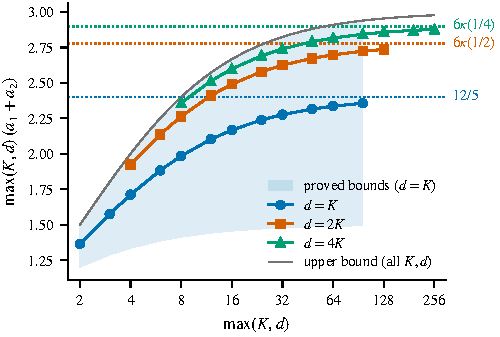
\includegraphics[width=0.92\columnwidth]{fig_constants.pdf}
\caption{The dimension factor of \cref{cor:dim}: $\max(K,d)(a_1+a_2)$ for three aspect ratios (exact values), the
proved bounds for square matrices (band; thin lines for the other ratios), and the proportional limits
$6\kappa(\gamma)$ (dotted).}
\label{fig:const}
\end{figure}

\textbf{Constants.} \cref{tab:const} and \cref{fig:const} give $q_{K,d}$, $a_1$, $a_2$, computed to high precision from the
exact formula for fractional moments of real Wishart matrices. In all $34$ sizes computed, $a_1<0<a_2$, the bounds
of \cref{cor:dim} hold, and $\max(K,d)(a_1+a_2)$ increases to the Marchenko--Pastur limit ($2.357$ at $96\times96$
against $\frac{12}5$).

\begin{figure*}[t]
\centering
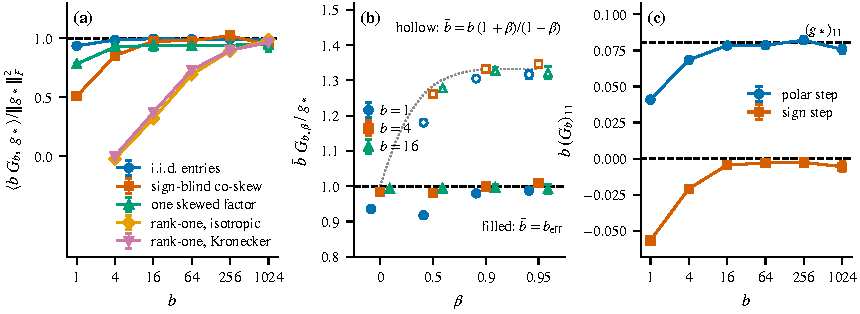
\includegraphics[width=\textwidth]{fig_law.pdf}
\caption{Tests of the first-order law on $2\times3$ matrices (zeros of the mean field, Monte Carlo with standard
errors). (a) $\inner{b\,G_b}{\gs}/\nF{\gs}^2$ for five noise laws; prediction: $1$. (b) Momentum: the zero for the
filtered noise, multiplied by a candidate effective batch size and divided by $\gs$; filled: $\beff$; hollow: the
variance-effective batch size; dotted: the predicted ratio $(1+\beta)^2/(1+\beta+\beta^2)$ of the two. (c) A noise law
whose entries have zero third cumulants: sign descent is unbiased to first order, the orthogonalized step is not.}
\label{fig:law}
\end{figure*}

\textbf{The law across noise laws} (\cref{fig:law}a). We compute the zero $G_b$ of $G\mapsto\E\polar(G+\xi_b)$ for
five laws on $\R^{2\times3}$: independent skewed entries; a ``sign-blind'' law with co-skewness only; one skewed
factor plus symmetric noise; and two rank-one laws $\delta x^\top$, with isotropic and with Kronecker covariance (for
the latter $\gs$ is evaluated from \eqref{eq:gs} by Monte Carlo). The ratio $\inner{bG_b}{\gs}/\nF{\gs}^2$ approaches
$1$ for four of the five laws: $0.990\pm0.003$ (i.i.d., $b\ge64$), $0.986\pm0.017$ (co-skew), $0.986\pm0.011$ and
$0.964\pm0.025$ (rank one, $b=1024$). For the one-factor law it stays at $0.94\pm0.02$ for all $b\ge16$, a deviation
of three standard errors that we cannot explain. Convergence is slow for the rank-one laws ($0.7$ at $b=64$; at
$b=4$ the isotropic one even has the opposite sign); we have no explanation for this either.

\textbf{Momentum} (\cref{fig:law}b). For exponentially filtered noise with $\beta\in\{0,0.5,0.9,0.95\}$ the zero
times $\beff$ is within $2\%$ of $\gs$ for $b\ge4$. Normalizing by the variance-effective batch size instead
gives $1.26$ to $1.35$, the predicted ratio $(1+\beta)^2/(1+\beta+\beta^2)$. The coupled iteration \eqref{eq:muon} on a
quadratic agrees with the zero of the frozen field (\cref{app:exp}).

\textbf{Sign-blind noise} (\cref{fig:law}c). For a law whose entries all have zero third cumulant but
$\E[\zeta_{11}\zeta_{12}^2]\ne0$, the sign step has no first-order offset (measured $b\,G_b$ compatible with $0$ for
$b\ge64$) and the polar step has the offset of \cref{cor:compare}: $0.078$ to $0.082$ measured for $b=16,\dots,256$
and $0.076\pm0.003$ at $b=1024$, against $0.0803$ predicted.

\begin{figure*}[t]
\centering
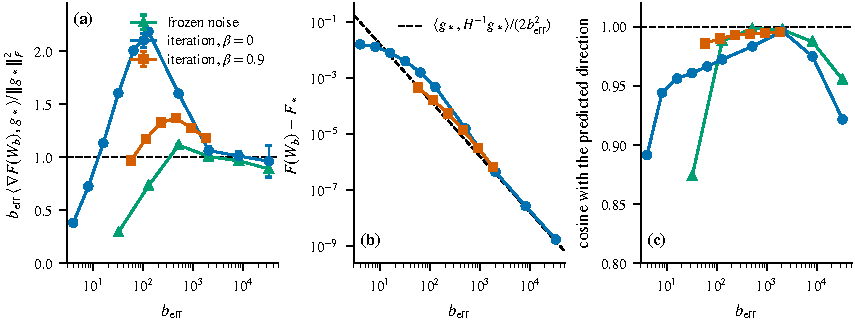
\includegraphics[width=\textwidth]{fig_digits.pdf}
\caption{Real data, no fitted parameter: least squares on \texttt{digits} ($W\in\R^{4\times16}$, $n=1797$,
minibatches with replacement). (a) The stationary gradient along the prediction, scaled by $\beff$; prediction: $1$.
Green: noise frozen at $W_\ast$ (\cref{thm:cf}); blue, red: limit of the iteration \eqref{eq:muon}, whose noise depends
on $W$ (compare \cref{thm:state}, which locates the zero of the mean field for $\beta=0$). (b) Excess loss at the limit against $\inner{\gs}{H^{-1}\gs}/(2\beff^2)$. (c) Cosine between
the measured and the predicted displacement.}
\label{fig:digits}
\end{figure*}

\textbf{A finite-sum problem on real data} (\cref{fig:digits}). We take ridge-regularized least squares on the
\texttt{digits} data set, with $16$ principal components as features and $4$ random projections of the one-hot
labels as targets, so that the covariance of the per-sample gradients is well conditioned. From the $1797$
per-sample gradients at the minimizer we compute $\Sigma$, $K_3$ and $\gs$ (by \eqref{eq:gs}; $\nnuc{\gs}=3.80\pm0.01$),
and compare with the limit of the iteration. The per-sample gradients have rank one and the noise depends on $W$,
so this tests \cref{thm:cf,thm:beff,thm:state} together, away from their idealizations. Three observations.
(i) \emph{The limit is the predicted one at large batch}: the scaled gradient along $\gs$ is $1.06\pm0.04$,
$1.01\pm0.05$, $0.96\pm0.15$ at $b=2048,8192,32768$ (batches larger than the data set, drawn with replacement), the
excess loss is $11$ to $15\%$ above $\inner{\gs}{H^{-1}\gs}/(2b^2)$ over these batch sizes, and the cosine with the
predicted direction reaches $0.997$. (ii) \emph{The approach is slow and not monotone}: the ratio is $0.38$, $0.72$ at
$b=4,8$, then for $16\le b\le512$ the stationary gradient overshoots the prediction, by a factor up to $2.2$ at
$b=128$ ($4.7$ in excess loss), while its direction is already right (cosine $0.97$). With the noise frozen at $W_\ast$
the ratio is $0.29$, $0.73$, $1.11$, $1.006\pm0.012$ at $b=32,128,512,2048$: most of the overshoot is therefore due to
the dependence of the noise on $W$, while a slower, also non-monotone approach remains for frozen noise. We
conjecture that the transient is governed by a second-order term in the dependence on $W$; we have no theory for
it. For reference, $\gs^\top\Sigma^{-1}\gs\approx26$ is the batch size at which the offset equals one standard deviation
of the noise; the transient lasts some $20$ to $80$ times longer. (iii) \emph{Momentum}: with $\beta=0.9$ the same
quantities are closer to the prediction at equal $\beff$ (ratio $0.97$ to $1.37$ for the gradient, $0.93$ to $1.86$ for
the excess loss), but the two curves do not collapse onto one function of $\beff$ in the transient regime. The
first-order law is thus an asymptotic statement whose range of validity, on this problem, is
$\beff\gtrsim2\cdot10^3$; below, it gives the direction and the order of magnitude.
}{\section{Experiments}\label{sec:exp}(pending)}

\section{Related work}\label{sec:related}

\textbf{Steepest descent and Muon.} Orthogonalized updates go back to stochastic spectral descent
\citep{carlson2015stochastic} and are analysed as steepest descent under the operator norm by \citet{bernstein2024old};
Muon is due to \citet{jordan2024muon}; see also \citet{lau2025polargrad,shulgin2026quadratic}. Complexity bounds for reaching approximate stationarity, and variance-reduced variants, are given in
\citet{huang2026muon,liu2025marsm}. The behaviour near optima under noise is
studied by \citet{xie2026muon}, \citet{chen2026when} and \citet{do2026muon}, who exhibit non-convergence and bound the
error; \citet{paquette2026phases} analyse high-dimensional dynamics. Our results are complementary: an asymptotically
exact first-order description of the limit point.

\textbf{Sign descent and medians.} That sign-based methods track medians rather than means is known
\citep{bernstein2019majority,chen2020distributed}; for other analyses of sign descent and its failure modes see
\citet{safaryan2021stochastic,balles2020geometry,karimireddy2019error}. Stochastic
algorithms for the geometric median are analysed by \citet{cardot2013efficient}; robustness properties of geometric
medians in \citet{minsker2015geometric,minskerstrawn}, and the distance between mean and geometric median in
\citet{schwank}. We are not aware of a previous study of the nuclear median; \cref{thm:two} computes its first-order
distance to the mean.

\textbf{Expansions.} \cref{thm:cf} is a multivariate Cornish--Fisher expansion \citep{cornish1938moments} for an
$M$-estimand with non-smooth score, proved with the Edgeworth expansion for functions of bounded oscillation
\citep[Thm.~20.1]{br}. Cumulants of linear filters are classical; their consequence for the bias, the skewness-effective batch size, is to
our knowledge new.
Stochastic mirror descent with Markov noise is treated in \citet{duchiemd}; our proof of \cref{thm:conv} is different
since the mirror structure is only approximate under momentum.

\section{Discussion and limitations}\label{sec:disc}

\textbf{What the law says in practice.} The stationary gradient of a Muon-type method is $\gs/\beff$: it decays like
$1/b$, is reduced by momentum by the factor $(1+\beta+\beta^2)/(1-\beta^2)$, and its direction is given by two moments
of the per-sample gradient noise when the covariance is isotropic, and in general by \eqref{eq:gs}, which can be
estimated from samples (\cref{sec:exp}). The associated excess loss is of order
$b^{-2}$, so at realistic batch sizes it is small relative to the variance-induced error of a constant step size; the
bias is the error that \emph{remains} when step sizes are annealed, and the one that variance reduction or large
batches act on.

\textbf{Limitations.} (1) The two-moment formula is exact for isotropic covariance $\sigma^2I$; for general $\Sigma$
the law holds with $\gs$ given by \eqref{eq:gs}, which we evaluate by Monte Carlo in \cref{sec:exp} but for which we
have no closed form. A Kronecker-factored extension is a natural next step. (2) The theory is for strongly convex
$F$; for deep networks it describes at best the local behaviour near a nondegenerate minimum. (3) \cref{thm:cf} assumes
Cram\'er's condition; the discrete case is the subject of \citet{companionII}. (4) We analyse the exact polar factor,
not its Newton--Schulz approximations \citep{do2026muon,shulgin2026quadratic}. (5) The proof of \cref{thm:a1} relies on exact
computer algebra for $K\ge3$. (6) \cref{thm:conv} assumes i.i.d.\ noise that does not depend on $W$, and
\cref{thm:state} locates zeros of the mean field without momentum; the finite-sum experiment of \cref{sec:exp} is
outside both, and it shows that the first-order regime can require large batches.

\section*{Impact Statement}
This paper presents work whose goal is to advance the theoretical understanding of optimization algorithms in machine
learning. We do not foresee specific societal consequences that must be highlighted here.

\bibliography{../../../theory/bias_law/shared/refs}
\bibliographystyle{icml2026}

\newpage
\appendix
\onecolumn

\section{Full statements}\label{app:full}
The main text states the results in compact form. The complete statements proved in this appendix are the following.

\begin{full}{Theorem}{thm:conv}\StmtConv\end{full}
\begin{full}{Theorem}{thm:cf}\StmtCF\end{full}
\begin{full}{Theorem}{thm:beff}\StmtBeff\end{full}
\begin{full}{Theorem}{thm:state}\StmtState\end{full}
\begin{proposition}[linear noise models]\label{prop:lin}\StmtLin\end{proposition}
\begin{full}{Theorem}{thm:two}\StmtTwo\end{full}
\begin{full}{Theorem}{thm:a1}\StmtAone\end{full}
\begin{full}{Corollary}{cor:dim}\StmtDim\end{full}
\begin{full}{Corollary}{cor:rank1}\StmtRankOne\end{full}
\begin{full}{Corollary}{cor:compare}\StmtCompare\end{full}

\section{The Gaussian side}\label{app:gauss}
% Module: Gaussian side (used by both papers). Labels: lem:gauss
\begin{lemma}[Gaussian side]\label{lem:gauss}
Let $\nu$ be a norm on $E$ with direction map $o$, and $\Sigma\succ0$. Write $\varphi_\Sigma$ for the density of
$Z_\Sigma\sim N(0,\Sigma)$ and $\He^\Sigma_k=(-1)^k\varphi_\Sigma^{-1}D^k\varphi_\Sigma$ for the Hermite tensors.
\begin{enumerate}
\item $\psi_\Sigma$ is $C^\infty$, $\Phi_\Sigma=\nabla\psi_\Sigma$ is odd, and the derivatives of $\Phi_\Sigma$ of every
order are bounded on $E$, uniformly for $\Sigma$ in a compact set of positive definite matrices.
\item For every symmetric $k$-tensor $\cK$ and every $x\in E$,
$\int o(x+y)\inner{\cK}{\He^\Sigma_k(y)}\varphi_\Sigma(y)\,dy=D^k\Phi_\Sigma(x)[\cK]$. In particular
$J_\Sigma=\E[o(Z_\Sigma)\otimes\Sigma^{-1}Z_\Sigma]$ and $T_\Sigma[\cK]=\E[o(Z_\Sigma)\inner{\cK}{\He_3^\Sigma(Z_\Sigma)}]$.
\item The even-order derivatives of $\Phi_\Sigma$ vanish at $0$.
\item $J_\Sigma$ is symmetric positive definite, and $\lambda_{\min}(J_\Sigma)$ is bounded below on compact sets of
positive definite $\Sigma$.
\item $J_{c\Sigma}=c^{-1/2}J_\Sigma$ and $T_{c\Sigma}=c^{-3/2}T_\Sigma$ for $c>0$; hence $\gs(c\Sigma,cK_3)=\gs(\Sigma,K_3)$
and $\gs$ is linear in $K_3$.
\item There is $c_0>0$, uniform on compact sets of $\Sigma$, with $|\Phi_\Sigma(h)|\ge c_0\min(|h|,1)$.
\end{enumerate}
\end{lemma}
\begin{proof}
A norm is Lipschitz, hence differentiable almost everywhere, with gradient $o$ wherever it is differentiable; so
$\nabla\psi_\Sigma(h)=\E\,o(h+Z_\Sigma)=\int o(y)\varphi_\Sigma(y-h)\,dy$ by dominated convergence, and one may
differentiate under the integral any number of times because $o$ is bounded: the $k$-th derivative is bounded by
$\sup|o|\int|D^k\varphi_\Sigma|$. This is (1), and $D_h^k[\varphi_\Sigma(y-h)]=(-1)^kD^k\varphi_\Sigma(y-h)
=\He_k^\Sigma(y-h)\varphi_\Sigma(y-h)$ gives (2) after the change of variable $y\mapsto x+y$. Oddness of $o$ and the
symmetry of $Z_\Sigma$ make $\Phi_\Sigma$ odd, whence (3). (5) follows from $o(tx)=o(x)$:
$\Phi_{c\Sigma}(h)=\Phi_\Sigma(h/\sqrt c)$.

(4) $J_\Sigma=\nabla^2\psi_\Sigma(0)$ is symmetric. Fix $v\ne0$, let
$s=\inner{\Sigma^{-1}v}{Z}/\inner v{\Sigma^{-1}v}$ and $Z'=Z-sv$; these are independent and $s\sim N(0,\tau^2)$ with
$\tau^{-2}=\inner v{\Sigma^{-1}v}$. Then $\psi_\Sigma(tv)+\E\nu(Z)=\E\,\hbar(s+t)$ with $\hbar(\varrho)=\E\nu(Z'+\varrho v)$
convex and $|\varrho|\nu(v)-\E\nu(Z')\le\hbar(\varrho)\le\E\nu(Z')+|\varrho|\nu(v)$. Hence the nondecreasing function
$\hbar'$ goes from $-\nu(v)$ to $\nu(v)$, the measure $d\hbar'$ has total mass $2\nu(v)>0$, and
$\inner{J_\Sigma v}v=\int\varphi_{\tau}\,d\hbar'>0$ because the Gaussian density $\varphi_\tau$ is positive. The lower
bound is uniform by continuity of $\Sigma\mapsto J_\Sigma$ and compactness.

(6) For a unit vector $\hat h$, $t\mapsto\inner{\Phi_\Sigma(t\hat h)}{\hat h}$ is nondecreasing by convexity of
$\psi_\Sigma$, and equals $t\inner{J_\Sigma\hat h}{\hat h}+O(t^3)$ near $0$ by (1) and (3), with uniform constants.
\end{proof}


\section{Proof of Theorem~\ref{thm:conv}}\label{app:conv}
% Module: convergence of norm-steepest descent with momentum, arbitrary square-integrable noise.
% Label: proof of thm:conv
\begin{proof}[Proof of Theorem~\ref{thm:conv}]
Let $K_\nu$ be the Lipschitz constant of $\nu$ for the Euclidean norm, so that $|O_t|\le K_\nu$, and let $L$, $\mu$ be
the smoothness and strong convexity constants of $F$. Extend the innovations to an i.i.d.\ sequence $(\xi_t)_{t\in\Z}$
and put $N_t=(1-\beta)\sum_{j\ge0}\beta^j\xi_{t-j}$: a stationary, square-integrable Markov chain with
$N_t=\beta N_{t-1}+(1-\beta)\xi_t$ and marginal law $\pi$, the law of $N_\beta$. Let $\mathcal F_t=\sigma(\xi_s,s\le t)$.
By induction $W_t$ and $G_t=\nabla F(W_t)$ are $\mathcal F_{t-1}$-measurable.

\emph{Step 1: the buffer tracks $G_t+N_t$.} Let $e_t=M_t-G_t-N_t$. Then $e_1=\beta(M_0-G_1-N_0)$ and, for $t\ge2$,
$e_t=\beta e_{t-1}+\beta(G_{t-1}-G_t)$ with $|G_t-G_{t-1}|\le LK_\nu\eta_{t-1}$. Hence
$|e_t|\le\beta^{t-1}|e_1|+LK_\nu\sum_{s<t}\beta^{t-s}\eta_s$ and, the lengths being nonincreasing,
\begin{equation}\label{eq:esum}
\sum_t\eta_t|e_t|\le|e_1|\,\eta_1\sum_t\beta^{t-1}+LK_\nu\sum_s\eta_s^2\sum_{t>s}\beta^{t-s}<\infty\qquad\text{almost surely.}
\end{equation}

\emph{Step 2: a pathwise inequality on loss differences.} Fix $a\in\mathcal A:=\arg\min\psi_{N_\beta}$, a nonempty convex
compact set, and let
\[
f_g(n)=\nu(g+n)-\nu(a+n),\qquad\hbar(g)=\int f_g\,d\pi=\psi_{N_\beta}(g)-\psi_{N_\beta}(a)\ \ge0 .
\]
The subgradient inequality for $\nu$ at the \emph{actual} argument $M_t=G_t+N_t+e_t$, tested against $a+N_t$, reads
$\nu(a+N_t)\ge\nu(M_t)+\inner{O_t}{a-G_t-e_t}$, whence
\begin{equation}\label{eq:path}
\inner{O_t}{G_t-a}\ \ge\ \nu(M_t)-\nu(a+N_t)-K_\nu|e_t|\ \ge\ f_{G_t}(N_t)-2K_\nu|e_t| .
\end{equation}
No regularity of the law of the noise and no choice of the subgradient enter here.

\emph{Step 3: Poisson equation.} Let $Q$ be the transition operator of $(N_t)$. For $j\ge0$,
$Q^jf_g(n)=\E f_g(\beta^jn+N^{(j)})$ with $N^{(j)}=(1-\beta)\sum_{i<j}\beta^i\xi_i$, and
$\hbar(g)=\E f_g(\beta^jN'+N^{(j)})$ with $N'\sim\pi$ independent. The function $n\mapsto f_g(n)$ is $2K_\nu$-Lipschitz
and $g\mapsto f_g(n)$ is $K_\nu$-Lipschitz, uniformly. Therefore, with $m_1=\E|N_\beta|$,
\[
\big|Q^jf_g(n)-\hbar(g)\big|\le2K_\nu\beta^j(|n|+m_1),\qquad
\big|[Q^jf_g(n)-\hbar(g)]-[Q^jf_{g'}(n)-\hbar(g')]\big|\le2K_\nu|g-g'| .
\]
Define $U_g(n)=\sum_{j\ge0}(Q^jf_g(n)-\hbar(g))$ and $V_g=QU_g=\sum_{j\ge1}(Q^jf_g-\hbar(g))$. The series converge
absolutely, $U_g-V_g=f_g-\hbar(g)$, both are jointly continuous in $(g,n)$, and, using
$\min(x,y)\le x^\alpha y^{1-\alpha}$ termwise, for every $\alpha\in(0,1)$,
\begin{equation}\label{eq:UV}
|U_g(n)|+|V_g(n)|\le C(1+|n|),\qquad|V_g(n)-V_{g'}(n)|\le C_\alpha|g-g'|^\alpha(1+|n|)^{1-\alpha},
\end{equation}
with constants depending on $K_\nu,\beta,m_1,\alpha$ but not on $g,g'$.

\emph{Step 4: the noise terms are summable.} We claim that $\sum_t\eta_t\big(f_{G_t}(N_t)-\hbar(G_t)\big)$ converges almost
surely. Write the summand, before multiplication by $\eta_t$, as
\[
\big[U_{G_t}(N_t)-V_{G_t}(N_{t-1})\big]+\big[V_{G_t}(N_{t-1})-V_{G_t}(N_t)\big].
\]
Since $G_t$ is $\mathcal F_{t-1}$-measurable and $\xi_t$ is independent of $\mathcal F_{t-1}$,
$\E[U_{G_t}(N_t)\mid\mathcal F_{t-1}]=V_{G_t}(N_{t-1})$: the first brackets are martingale differences, with second
moments bounded by $C\,\E(1+|N_\beta|)^2$ uniformly in $t$ by \eqref{eq:UV} (no bound on $G_t$ is needed). As
$\sum_t\eta_t^2<\infty$, their weighted sum converges almost surely. For the second brackets, summation by parts gives
\[
\sum_{t=1}^T\eta_t\big[V_{G_t}(N_{t-1})-V_{G_t}(N_t)\big]=\eta_1V_{G_1}(N_0)-\eta_TV_{G_T}(N_T)
+\sum_{t=1}^{T-1}\big[\eta_{t+1}V_{G_{t+1}}(N_t)-\eta_tV_{G_t}(N_t)\big].
\]
The boundary term $\eta_TV_{G_T}(N_T)$ tends to $0$ almost surely because $\sum_T\eta_T^2\E(1+|N_T|)^2<\infty$. By
\eqref{eq:UV} and $|G_{t+1}-G_t|\le LK_\nu\eta_t$, the $t$-th internal difference is at most
$C(\eta_t-\eta_{t+1})(1+|N_t|)+C_\alpha\eta_t^{1+\alpha}(1+|N_t|)^{1-\alpha}$ in absolute value; choosing
$\alpha\in(\frac1\theta-1,1)$, which is possible because $\theta>\frac12$, the expectations are summable. This proves the
claim.

\emph{Step 5: Lyapunov function.} Let $W^a=(\nabla F)^{-1}(a)$ (strong convexity makes $\nabla F$ a bijection of $E$ with
a $\frac1\mu$-Lipschitz inverse) and $B_t(a)=F(W_t)-F(W^a)-\inner a{W_t-W^a}\ge\frac\mu2|W_t-W^a|^2$. Smoothness of $F$ and
\eqref{eq:path} give
\[
B_{t+1}(a)\le B_t(a)-\eta_t\inner{O_t}{G_t-a}+\tfrac L2K_\nu^2\eta_t^2
\le B_t(a)-\eta_t\hbar(G_t)-\eta_t\big(f_{G_t}(N_t)-\hbar(G_t)\big)+2K_\nu\eta_t|e_t|+\tfrac L2K_\nu^2\eta_t^2 .
\]
By \eqref{eq:esum} and Step 4 the series of the last three terms converges almost surely; subtracting its partial sums
from $B_t(a)+\sum_{s<t}\eta_s\hbar(G_s)$ gives a nonincreasing sequence bounded below. Hence $B_t(a)$ converges and
$\sum_t\eta_t\hbar(G_t)<\infty$. In particular $(W_t)$ and $(G_t)$ are bounded and, as $\sum_t\eta_t=\infty$, there is a
cluster point $\widehat G$ of $(G_t)$ with $\hbar(\widehat G)=0$, i.e.\ $\widehat G\in\mathcal A$.

\emph{Step 6: a single limit.} Almost surely the above holds simultaneously for all $a$ in a countable dense subset of
$\mathcal A$. On bounded sets of $W$ the maps $a\mapsto F(W)-F(W^a)-\inner a{W-W^a}$, $a\in\mathcal A$, are equicontinuous,
so $B_t(a)$ converges for every $a\in\mathcal A$, in particular for $a=\widehat G$. Along the subsequence defining
$\widehat G$, $W_t\to W^{\widehat G}$ and $B_t(\widehat G)\to0$; hence $B_t(\widehat G)\to0$ along the whole sequence, and
$W_t\to W^{\widehat G}$, $G_t\to\widehat G$.
\end{proof}


\section{Proofs of Theorems~\ref{thm:cf}, \ref{thm:beff} and~\ref{thm:state}}\label{app:cf}
% Module: first-order law under Cramer's condition. Labels: lem:osc, lem:edge, proof of thm:cf, proof of thm:beff
\begin{lemma}[oscillation]\label{lem:osc}
For the $\ell_1$, Euclidean and nuclear norms with their direction maps, and every compact set $\mathcal C$ of positive
definite covariances, there is $C$ such that for $\varepsilon\le1$
\[
\sup_{\Sigma\in\mathcal C}\ \sup_{y\in E}\ \E\,\mathrm{osc}\big(o;B(y+Z_\Sigma,\varepsilon)\big)\le C\varepsilon\log(e/\varepsilon),
\]
where $\mathrm{osc}(o;B)$ is the largest oscillation on $B$ of a coordinate of $o$. Moreover
$\sup_y\Prob(\sigma_{\min(K,d)}(y+Z_\Sigma)\le t)\le Ct$.
\end{lemma}
\begin{proof}
$\ell_1$: the oscillation vanishes unless some coordinate of $y+Z$ is within $\varepsilon$ of $0$, an event of
probability at most $N\varepsilon\sup\varphi$. Euclidean: $\mathrm{osc}\le\min(2,2\varepsilon/(|x|-\varepsilon)_+)$.
Nuclear, $K\le d$ (transpose otherwise): with rows $\varrho_j$ of $X$,
$\sigma_K(X)\ge K^{-1/2}\min_j\dist(\varrho_j,\operatorname{span}\{\varrho_l\}_{l\ne j})$; conditionally on the other rows,
$\varrho_j$ is Gaussian with covariance at least $\lambda_{\min}(\Sigma)I$ and its component along a unit normal to the
span has a density bounded by $(2\pi\lambda_{\min})^{-1/2}$; a union bound gives the small-ball estimate. By
\citet{lisun}, $\nF{\polar(A)-\polar(B)}\le2\nF{A-B}/(\sigma_K(A)+\sigma_K(B))$ for $A,B$ of rank $K$; hence
$\mathrm{osc}(\polar;B(x,\varepsilon))\le\min(2,4\varepsilon/\sigma_K(x))$ when $\sigma_K(x)>2\varepsilon$, and
$\E\min(2,4\varepsilon/\sigma_K)\le C\varepsilon\log(e/\varepsilon)$.
\end{proof}

\begin{lemma}[one-term expansion of the mean field, uniform in the shift]\label{lem:edge}
Under Assumption~\ref{ass:N}, for the norms of Lemma~\ref{lem:osc}, with $X_b=\sqrt b\,\xi_b$,
\[
\sup_{h\in E}\Big|\E\,o(X_b+h)-\Phi_\Sigma(h)-\frac1{6\sqrt b}\,D^3\Phi_\Sigma(h)[K_3]\Big|=o(b^{-1/2}).
\]
\end{lemma}
\begin{proof}
Theorem~20.1 of \citet{br} with $s=3$ provides $\delta_b=o(b^{-1/2})$ and $c,c'>0$, depending on the law of $\zeta$ only,
such that for every bounded Borel $f$,
$|\int f\,d(Q_b-\Phi_{0,\Sigma}-b^{-1/2}P_1)|\le\sup|f|\,\delta_b+c'\sup_y\int\mathrm{osc}(f;B(x+y,2e^{-cb}))\varphi_\Sigma(x)dx$,
where $Q_b$ is the law of $X_b$ and $P_1$ has density $\frac16\inner{K_3}{\He_3^\Sigma}\varphi_\Sigma$. Apply it to the
coordinates of $f=o(\cdot+h)$: the supremum is bounded, the oscillation term is $O(be^{-cb})$ by Lemma~\ref{lem:osc},
uniformly in $h$, and $\int o(x+h)\frac16\inner{K_3}{\He^\Sigma_3(x)}\varphi_\Sigma(x)dx=\frac16D^3\Phi_\Sigma(h)[K_3]$ by
Lemma~\ref{lem:gauss}(2).
\end{proof}

\begin{proof}[Proof of Theorem~\ref{thm:cf}]
By homogeneity $\Phi_{\xi_b}(G)=\E\,o(X_b+\sqrt b\,G)$. Let $G=(\gs+u)/b$ with $|u|\le R$, so $h=\sqrt bG=O(b^{-1/2})$.
By Lemma~\ref{lem:gauss}, $\Phi_\Sigma(h)=J_\Sigma h+O(|h|^3)$ and $D^3\Phi_\Sigma(h)[K_3]=T_\Sigma[K_3]+O(|h|^2)$; with
Lemma~\ref{lem:edge},
\[
\Phi_{\xi_b}(G)=b^{-1/2}\big(J_\Sigma(\gs+u)+\tfrac16T_\Sigma[K_3]\big)+o(b^{-1/2})=b^{-1/2}J_\Sigma u+o(b^{-1/2}),
\]
uniformly in $|u|\le R$. Take $|u|=\epsilon$: $\inner{\Phi_{\xi_b}(G)}{u}\ge b^{-1/2}(\lambda_{\min}(J_\Sigma)\epsilon^2-o(1))>0$
for $b\ge b_0(\epsilon)$. If a minimizer $G'$ of $\psi_{\xi_b}$ had $|G'-\gs/b|>\epsilon/b$, let $G$ be the point of the
segment $[\gs/b,G']$ on the sphere of radius $\epsilon/b$, so that $G'-G=\tau u$ with $\tau>0$; since
$\Phi_{\xi_b}(G)\in\partial\psi_{\xi_b}(G)$, $\psi_{\xi_b}(G')\ge\psi_{\xi_b}(G)+\tau\inner{\Phi_{\xi_b}(G)}u>\psi_{\xi_b}(G)$,
a contradiction.
\end{proof}

\begin{proof}[Proof of Theorem~\ref{thm:beff}]
Write the filtered noise as a batch mean of regrouped samples:
$N_w=\sum_kw_k\xi_b^{(k)}=\frac1b\sum_{i\le b}Y_i$ with $Y_i=\sum_kw_k\zeta_{k,i}$ i.i.d. The series converges absolutely in
$L^3$ because $\sum_k|w_k|<\infty$; cumulants add over independent summands, so $Y$ has mean $0$, covariance
$\rho_2\Sigma$ and third cumulant $\rho_3K_3$; and $|\E e^{i\inner tY}|=\prod_k|\varphi(w_kt)|\le|\varphi(w_{k_0}t)|$ for an
index with $w_{k_0}\ne0$, so $Y$ satisfies Cram\'er's condition. Theorem~\ref{thm:cf} applies to $Y$ and gives
$\arg\min\psi_{N_w}\subset B\big(\gs(\rho_2\Sigma,\rho_3K_3)/b,\,o(1/b)\big)$, and
$\gs(\rho_2\Sigma,\rho_3K_3)=\frac{\rho_3}{\rho_2}\gs(\Sigma,K_3)$ by Lemma~\ref{lem:gauss}(5). For the exponential
average, $\rho_p=(1-\beta)^p/(1-\beta^p)$ and $\rho_3/\rho_2=(1-\beta^2)/(1+\beta+\beta^2)$.
\end{proof}

% Module: parameter-dependent noise. Label: eq:hb
\begin{proof}[Proof of Theorem~\ref{thm:state}]
By homogeneity and (iii), uniformly in $W\in\mathcal U$,
\begin{equation}\label{eq:hb}
h_b(W)=\Phi_{\Sigma(W)}\big(\sqrt b\,\nabla F(W)\big)+\tfrac1{6\sqrt b}D^3\Phi_{\Sigma(W)}\big(\sqrt b\,\nabla F(W)\big)[K_3(W)]+o(b^{-1/2}).
\end{equation}
\emph{Step 1.} By Lemma~\ref{lem:gauss}, uniformly over the compact set of covariances,
$|\Phi_{\Sigma(W)}(h)|\ge c_0\min(|h|,1)$ and the second term of \eqref{eq:hb} is at most $C_1b^{-1/2}$. Hence
$|h_b(W)|\le\delta b^{-1/2}$ forces $c_0\min(\sqrt b|\nabla F(W)|,1)\le(C_1+\delta+o(1))b^{-1/2}$, i.e.\
$|\nabla F(W)|\le C_2/b$ and $|W-W_\ast|\le C_3/b$ for $b$ large. \emph{Step 2.} Write $W=W_\ast+w/b$, $|w|\le C_3$. Then
$\sqrt b\,\nabla F(W)=b^{-1/2}(Hw+o(1))$, $\Sigma(W)\to\Sigma_\ast$, $K_3(W)\to K_{3\ast}$, and $J_\Sigma$, $T_\Sigma$ are
continuous in $\Sigma$, so \eqref{eq:hb} reads $h_b(W)=b^{-1/2}\big(J_{\Sigma_\ast}Hw+\frac16T_{\Sigma_\ast}[K_{3\ast}]+o(1)\big)$,
uniformly in $|w|\le C_3$. If $|h_b(W)|\le\delta b^{-1/2}$ then $|w-H^{-1}\gs|\le\|(J_{\Sigma_\ast}H)^{-1}\|(\delta+o(1))$.
\emph{Existence.} The continuous field $w\mapsto\sqrt b\,h_b(W_\ast+w/b)$ converges uniformly on a ball around
$H^{-1}\gs$ to the affine isomorphism $w\mapsto J_{\Sigma_\ast}H(w-H^{-1}\gs)$, which has degree $\pm1$ there.
\end{proof}

\begin{proof}[Proof of Proposition~\ref{prop:lin}]
Apply Theorem~20.1 of \citet{br} to $\chi$ and to $f_{W,h}(x)=o(L_Wx+h)$: its oscillation on a ball of radius
$\varepsilon$ is that of $o$ on a ball of radius $\|L_W\|\varepsilon$ around $L_Wx+h$, and $L_WZ_\chi\sim
N(0,\Sigma(W))$ with $\Sigma(W)=L_W\Sigma_\chi L_W^\top$ in a compact set of positive definite matrices, so
Lemma~\ref{lem:osc} bounds the oscillation term uniformly; the remainder $\delta_b$ depends on $\chi$ only. The
Gaussian and first Edgeworth terms of $\chi$ push forward to those of covariance $\Sigma(W)$ and cumulant
$L_W^{\otimes3}K_3^\chi=K_3(W)$: with $u(s)=\E f_{W,h}(Z_\chi+s)=\Phi_{\Sigma(W)}(h+L_Ws)$,
$-\int f_{W,h}K_3^\chi\cdot\partial^3\varphi_{\Sigma_\chi}=D^3u(0)[K_3^\chi]=D^3\Phi_{\Sigma(W)}(h)[L_W^{\otimes3}K_3^\chi]$.
\end{proof}

\paragraph{The excess loss.} With $W_b-W_\ast=\frac1bH^{-1}\gs+o(1/b)$ and $F$ twice differentiable at $W_\ast$,
$F(W_b)-F(W_\ast)=\frac12\inner{W_b-W_\ast}{H(W_b-W_\ast)}+o(|W_b-W_\ast|^2)=\frac1{2b^2}\inner{\gs}{H^{-1}\gs}+o(b^{-2})$.

\section{Proof of Theorem~\ref{thm:two} and of the corollaries}\label{app:two}
% Module: two-moment theorem (proof), counting lemma, proofs of corollaries. Labels: lem:count
\begin{proof}[Proof of Theorem~\ref{thm:two}]
\emph{(a) Reduction.} $J_I$ and $T_I$ are equivariant under $Z\mapsto UZV^\top$, $U\in O(K)$, $V\in O(d)$, because
$\polar(UZV^\top)=U\polar(Z)V^\top$ and the law of $Z$ is invariant. $E=\R^K\otimes\R^d$ is irreducible, so
$J_I=c\,\mathrm{Id}$ with $c=\tr J_I/N=\E\inner{\polar(Z)}Z/N=c_{K,d}$ \citep{xie2026muon,chen2026when}. $T_I$ is an invariant element of
$E^{\otimes4}=(\R^K)^{\otimes4}\otimes(\R^d)^{\otimes4}$; the invariants of $O(K)\times O(d)$ are spanned by the
products $\pi\otimes\pi'$ of an $O(K)$-invariant and an $O(d)$-invariant, and by the first fundamental theorem for the
orthogonal group each factor is spanned by the three pairings of the four indices. Label a pairing by the input slot
paired with the output index; $T_I$ is symmetric in its three input slots, the symmetric group $S_3$ permutes the nine
products $(\pi,\pi')$ with two orbits, $\{\pi=\pi'\}$ and $\{\pi\ne\pi'\}$, and the orbit averages are the tensors of
$\cA$ and $\cB$ on symmetric arguments. Hence $T_I=\alpha\cA+\beta\cB$. To find $\alpha,\beta$ contract with one representative of each orbit:
using $\He_3(Z)^{(ab),(cd),(ef)}=Z_{ab}Z_{cd}Z_{ef}-Z_{ab}\delta_{(cd),(ef)}-Z_{cd}\delta_{(ab),(ef)}-Z_{ef}\delta_{(ab),(cd)}$,
\begin{align*}
\textstyle\sum_{ij}\cA\big[\E\,\polar(Z)_{ij}\He_3(Z)\big]_{ij}&=\E\big[\nnuc Z(\nF Z^2-N-2)\big]=-m_1,\\
\textstyle\sum_{ij}\cB\big[\E\,\polar(Z)_{ij}\He_3(Z)\big]_{ij}&=\E\big[\inner{\polar(Z)}{ZZ^\top Z}\big]-(K+d+1)m_1=m_3-(K+d+1)m_1,
\end{align*}
where $\E[\nnuc Z\nF Z^2]=(N+1)m_1$ because $\nF Z$ is independent of $Z/\nF Z$ and $\E\chi_N^3=(N+1)\E\chi_N$. On the
other side, by Lemma~\ref{lem:count}, the same contractions of $\alpha\cA+\beta\cB$ are
$\frac N3[(N+2)\alpha+(K+d+1)\beta]$ and $\frac N3[(K+d+1)\alpha+\frac12(N+K+d+3)\beta]$. The determinant of this system
is $\frac{N^2}{18}(K-1)(d-1)(K+2)(d+2)$; solving, and substituting $m_3=(K+d-q)m_1$ from (b), gives
$\alpha=-c_{K,d}a_1$, $\beta=-c_{K,d}a_2$ with \eqref{eq:a12}. Then \eqref{eq:two} is Theorem~\ref{thm:cf} with the scaling
of Lemma~\ref{lem:gauss}. The map $K_3\mapsto(\cA[K_3],\cB[K_3])$ is onto $E\oplus E$ (the two equivariant maps are
linearly independent and $E$ is irreducible), so $K_3\mapsto a_1\cA+a_2\cB$ is onto $E$.

\emph{(b)} $\sum_is_i^3=\inner Z{f(Z)}$ with the spectral function $f(Z)=(ZZ^\top)^{1/2}Z=U\operatorname{diag}(s_i^2)V^\top$,
which is locally Lipschitz with derivative of polynomial growth; by Stein's identity $m_3=\E\operatorname{div}f(Z)$ and by the divergence formula for spectral functions
\citep{candes}, with $\varphi(s)=s^2$,
$\operatorname{div}f=\sum_i\big(\varphi'(s_i)+|K-d|\frac{\varphi(s_i)}{s_i}\big)+\sum_{i\ne j}\frac{s_i\varphi(s_i)-s_j\varphi(s_j)}{s_i^2-s_j^2}
=(K+d)\sum_is_i-\sum_{i\ne j}\frac{s_is_j}{s_i+s_j}$, since
$\frac{s_i^3-s_j^3}{s_i^2-s_j^2}=s_i+s_j-\frac{s_is_j}{s_i+s_j}$. The bounds on $q$ follow from
$0<\frac{s_is_j}{s_i+s_j}<\frac{s_i+s_j}4$ almost surely, and $a_2>0$ from \eqref{eq:a12}.

\emph{(c)} Algebra from \eqref{eq:a12}, using $Kd+1-(K+d)=(K-1)(d-1)$ and, for $K\le d$,
$Kd+2-K(K+d+1)=-(K-1)(K+2)$; positivity from $q<\frac{r-1}2\le\frac{\bar d-1}2$.

\emph{(d)} $\nabla^4\psi_I(0)[D,D,D,D]=\inner D{T_I[D^{\otimes3}]}$, $\cA[D^{\otimes3}]=\nF D^2D$,
$\cB[D^{\otimes3}]=DD^\top D$. If $a_1\ge0$ the sign is clear. If $a_1<0$, $\nF D^4\le\operatorname{rank}(D)\tr(DD^\top)^2$
gives $a_1\nF D^4+a_2\tr(DD^\top)^2\ge(r\,a_1+a_2)\tr(DD^\top)^2>0$ by (c).

\emph{(e)} The empirical distribution of the $s_i^2/d$ converges almost surely to the Marchenko--Pastur law of ratio
$\gamma$, with convergence of the moments $m_1/(K\sqrt d)$ and $m_3/(Kd^{3/2})$ (the extreme singular values are bounded in
every $L^p$); by (b), $q/K=(K+d)/K-m_3/(Km_1)\to[(1+\gamma)\mu_{1/2}-\mu_{3/2}]/(\gamma\mu_{1/2})$. Here $\mu_{1/2}(1)=\frac8{3\pi}$, $\mu_{3/2}(1)=\frac{64}{15\pi}$
(quarter-circle law), hence $\kappa(1)=2-\frac85$. The limits of $a_1,a_2$ follow from \eqref{eq:a12}.

\emph{$K=1$.} The same computation with a single invariant; $m_3=(d+1)m_1$ and the contraction of the invariant with
itself is $N(N+2)/3$, so $\alpha+\beta=-3m_1/(d(d+2))$.
\end{proof}

\begin{lemma}[counting]\label{lem:count}
Let $\mathsf A_1$, $\mathsf B_1$ be one pairing tensor from each orbit and $\bar{\mathsf A}$, $\bar{\mathsf B}$ the orbit
averages (so that $\bar{\mathsf A}$, $\bar{\mathsf B}$ are the tensors of $\cA$, $\cB$ on symmetric arguments). Then
$\inner{\mathsf A_1}{\bar{\mathsf A}}=\frac{N(N+2)}3$, $\inner{\mathsf A_1}{\bar{\mathsf B}}=\inner{\mathsf B_1}{\bar{\mathsf A}}=\frac{N(K+d+1)}3$,
$\inner{\mathsf B_1}{\bar{\mathsf B}}=\frac{N(N+K+d+3)}6$.
\end{lemma}
\begin{proof}
The inner product of two pairing tensors is $K^{\ell}d^{\ell'}$, $\ell,\ell'\in\{1,2\}$ being the numbers of closed
loops of row and of column indices. The three inner products of $\mathsf A_1$ with the first orbit are $N^2,N,N$; its
six inner products with the second orbit are $Kd^2,Kd^2,K^2d,K^2d,Kd,Kd$; the six inner products of $\mathsf B_1$ with
its orbit are $K^2d^2,K^2d,Kd^2,Kd,Kd,Kd$. (Direct enumeration; also verified by brute-force contraction for seven sizes.)
\end{proof}

\begin{proof}[Proof of Corollary~\ref{cor:dim}]
For independent entries the only nonzero components of $K_3$ are $K_3^{(ij),(ij),(ij)}=\kappa_3$, so
$\cA[K_3]_{ij}=\cB[K_3]_{ij}=\kappa_3$. The value of $a_1+a_2$ is Theorem~\ref{thm:two}(c); the upper bound is
$q_{K,d}<\frac{r-1}2$ with $(r+2)(\bar d+2)=(K+2)(d+2)$, and the lower bound is Theorem~\ref{thm:a1}.
\end{proof}

\begin{proof}[Proof of Corollary~\ref{cor:rank1}]
If $\zeta=uv^\top$ then $\zeta\zeta^\top\zeta=|u|^2|v|^2uv^\top=\nF\zeta^2\zeta$, so $\cB=\cA$ and
$\gs=(a_1+a_2)\cA/(6\sigma^2)$. For the Frobenius norm apply the case $K=1$ of Theorem~\ref{thm:two} on $\R^{Kd}$:
$\gs=\frac3{Kd+2}\cA/(6\sigma^2)$. The ratio is $\varrho=\frac{(3+2q)(Kd+2)}{(K+2)(d+2)}$; it exceeds
$\frac{Kd+2}{K+d+1}>1$ by Theorem~\ref{thm:a1} (as $Kd+2-(K+d+1)=(K-1)(d-1)>0$), and it is below
$\frac{(r+2)(Kd+2)}{(K+2)(d+2)}=\frac{Kd+2}{\bar d+2}<r$.
\end{proof}

\begin{proof}[Proof of Corollary~\ref{cor:compare}]
(i) Theorems~\ref{thm:cf} and~\ref{thm:two}; for the $\ell_1$ norm and diagonal $\Sigma$,
$J=\operatorname{diag}(\sqrt{2/\pi}/\sigma_k)$ and $T[K_3]_k=-\sqrt{2/\pi}\,\kappa_{3,k}/\sigma_k^3$, so
$(\gs)_k=\kappa_{3,k}/(6\sigma_k^2)$. (ii) The only nonzero entries of $K_3$ are the permutations of
$((11),(12),(12))$, whence $\cA=\cB=\tau e_1e_1^\top$. Such a law exists:
$\zeta_{11}=\varrho(\zeta_{12}^2-1)/\sqrt2+\sqrt{1-\varrho^2}\,\epsilon$ with $\epsilon$ an independent centred variable
(minus a centred Gamma variable when $\varrho>0$) whose third moment cancels that of the first term. (iii) For this tensor
$\cA_{11}=1+K_3^{(11),(22),(22)}$, $\cB_{11}=1$ and all other entries of $\cA,\cB$ vanish (the pattern
$(kj),(kl),(il)$ of $\cB$ is never a permutation of $((11),(22),(22))$), so
$a_1\cA+a_2\cB=(a_1+a_2+a_1K_3^{(11),(22),(22)})e_1e_1^\top=0$; a small multiple of this $K_3$ is the third cumulant of a law
with covariance $I$ and a density (the pairs of covariance and third moment of laws with a density near the Gaussian
fill a neighbourhood of $(I,0)$). (iv) Cumulants add over independent summands, and
$a_1\nF M^4+a_2\tr(MM^\top)^2>0$ by Theorem~\ref{thm:two}(d).
\end{proof}


\section{Proof of Theorem~\ref{thm:a1}}\label{app:a1}
% Module: sign of a_1 (computer-assisted for K>=3). Label: eq:num
\begin{proof}[Proof of Theorem~\ref{thm:a1}]
Let $W=ZZ^\top$, $D_p=\E\tr W^{p/2}=\E\sum_is_i^p$, $r(p)=D_{p+2}/D_p$ and $m=K+d+1$.
\emph{Equivalences.} By the Stein identity $D_3=(K+d-q)D_1$ of Theorem~\ref{thm:two}(b), the claim is
$D_3<c^\ast D_1$ with $c^\ast=K+d-\frac{(K-1)(d-1)}{2m}$. Since $\E[\tr W\cdot\sum_js_j^p]=(Kd+p)D_p$ (differentiate the
Gaussian integral along dilations), $\E\sum_js_j^pA_j/D_p=Kd+p-r(p)$; and $r(2)=m$,
$r(4)=\E\tr W^3/\E\tr W^2=(K^2+d^2+3Kd+3K+3d+4)/m$, so $3r(2)-r(4)=2c^\ast$: this is (i) and (ii). (iii):
$\E_\varpi[x^{\pm1/2}]=D_{2\pm1}/(Kd)$, $\E_\varpi x=m$, $\E_\varpi x^2=\E\tr W^3/(Kd)$, and $m-\frac v{2m}=c^\ast$. For a Gamma law
of shape $\alpha$ and scale $\theta$ both sides of (iii) equal $\theta(\alpha-\frac12)$; for $K=1$, $\varpi$ is the $\chi^2_{d+2}$ law.

\emph{$K=2$.} The density of $(s_1>s_2)$ is proportional to $(s_1^2-s_2^2)(s_1s_2)^{d-2}e^{-(s_1^2+s_2^2)/2}$. With
$s_1+s_2=\rho\cos\frac\phi2$, $s_1-s_2=\rho\sin\frac\phi2$, $\phi\in(0,\frac\pi2)$, the variables $\rho$ and
$\gamma=\cos\phi$ are independent, $\gamma$ has density $(d-1)\gamma^{d-2}$ on $(0,1)$,
$\sum s_i=\rho\sqrt{(1+\gamma)/2}$ and $\frac{2s_1s_2}{s_1+s_2}=\rho\gamma/\sqrt{2(1+\gamma)}$. Hence
$q_{2,d}=\E[\gamma(1+\gamma)^{-1/2}]/\E[(1+\gamma)^{1/2}]$ (for $d=2$: $q_{2,2}=(3\sqrt2-2)/7$), and with $n=d-2$ the claim
is $\mathcal F=\int_0^1\gamma^n\big((n+9)\gamma-(n+1)\big)(1+\gamma)^{-1/2}d\gamma>0$. Integrating by parts,
$(n+1)\int_0^1\gamma^n(1+\gamma)^{-1/2}=2^{-1/2}+\frac12\int_0^1\gamma^{n+1}(1+\gamma)^{-3/2}$, so
$\mathcal F\ge(n+\frac{17}2)\int_0^1\gamma^{n+1}(1+\gamma)^{-1/2}d\gamma-2^{-1/2}\ge2^{-1/2}\big(\frac{n+17/2}{n+2}-1\big)>0$.

\emph{$K\ge3$.} By (iii) the claim is $\E_\varpi[g]>0$ for $g(x)=(c^\ast-x)x^{-1/2}$. For $n\ge1$, $g^{(n)}$ has the sign
$(-1)^n$ on $(0,\infty)$; so (1)~the Taylor polynomial $T_5$ of $g$ at $m$ satisfies $g\ge T_5$, and (2)~the Hermite
interpolant $H$ of $g$ at four nodes (values and first derivatives) satisfies $g\ge H$. Both $\E_\varpi T_5$ and $\E_\varpi H$
are linear in the moments $\E_\varpi x^j=\E\tr W^{j+1}/(Kd)$, $j\le7$, and $\E\tr W^k$ is a polynomial in $(K,d)$ computed by
Wick's formula (sum over the $(2k-1)!!$ pairings of $K^{\#\text{row classes}}d^{\#\text{column classes}}$). Step~1:
\begin{equation}\label{eq:num}
\begin{aligned}
\sqrt m\,\E_\varpi T_5&=\mathrm{NUM}(K,d)/(256\,m^6),\\
\mathrm{NUM}&=K^5(112d^2+112d-224)+K^4(266d^3-221d^2-3854d-3751)\\
&+K^3(266d^4-358d^3-10520d^2-33316d-36712)\\
&+K^2(112d^5-221d^4-10520d^3-52379d^2-118790d-96410)\\
&+K(112d^5-3854d^4-33316d^3-118790d^2-166352d-64872)\\
&-224d^5-3751d^4-36712d^3-96410d^2-64872d+16497,
\end{aligned}
\end{equation}
and $\mathrm{NUM}(9+\alpha,9+\alpha+\beta)$, $\mathrm{NUM}(3,22+\beta)$, $\mathrm{NUM}(4,17+\beta)$, $\mathrm{NUM}(5,14+\beta)$,
$\mathrm{NUM}(6,12+\beta)$, $\mathrm{NUM}(7,11+\beta)$, $\mathrm{NUM}(8,9+\beta)$ are polynomials in $\alpha,\beta$ with
positive coefficients. Step~2: for the $52$ remaining pairs $3\le K\le d$ ($K=3$, $d\le21$; $K=4$, $d\le16$; $K=5$,
$d\le13$; $K=6$, $d\le11$; $K=7$, $d\le10$; $(8,8)$), nodes $x_i=t_i^2$ with rational $t_i$ (so that $g(x_i),g'(x_i)$
are rational; we take $t_i$ to be $\sqrt{z_i}$ rounded to the nearest multiple of $\frac1{16}$, where $z_1<\dots<z_4$ are the
nodes of the four-point Gauss quadrature of $\varpi$, but any four distinct positive rationals for which the value is
positive would do) give exact rational values $\E_\varpi H>0$, the smallest being $0.0323$ at $(3,21)$. Both steps are exact
integer computations; the moment polynomials, the identity \eqref{eq:num}, the positivity of the coefficients and the
$52$ certificates were recomputed by two independent implementations (supplementary code, \texttt{a1/} and \texttt{lattice/v01, v02}).
Finally $a_1<0$ is equivalent to $a_1+a_2>\frac3{K+d+1}$: by Theorem~\ref{thm:two}(c),
$a_1+a_2-\frac3{K+d+1}=\frac{6}{(K+2)(d+2)}\big(q_{K,d}-\frac{(K-1)(d-1)}{2(K+d+1)}\big)$, because
$3+\frac{(K-1)(d-1)}{K+d+1}=\frac{(K+2)(d+2)}{K+d+1}$.
\end{proof}


\IfFileExists{exp_appendix.tex}{\section{Details of the numerical experiments}\label{app:exp}

\paragraph{Constants.} $q_{K,d}=K+d-m_3/m_1$ with $m_p=\E\tr(ZZ^\top)^{p/2}$ evaluated by the Pfaffian formula for
moments of real Wishart matrices, in multiprecision arithmetic, the working precision being raised until the known
value $\E\tr(ZZ^\top)^2=Kd(K+d+1)$ is reproduced to $10^{-25}$; $q_{2,2}$ agrees with $(3\sqrt2-2)/7$ to $16$ digits and
all values agree with direct Monte Carlo.

\paragraph{Zeros of mean fields.} For a noise law and a batch size $b$, batch means are sampled exactly and the zero of
the sampled field $G\mapsto\frac1S\sum_s\polar(G+\xi^{(s)})$ is computed with common random numbers; standard errors
come from independent blocks. For momentum the filtered noise is sampled from its stationary law (truncated
geometric series). The five laws of \cref{fig:law}(a) are on $\R^{2\times3}$: (1) independent entries
$\mathrm{Exp}(1)-1$; (2) a law with $\E\zeta_{ij}^3=0$ for all entries and $\E[\zeta_{11}\zeta_{12}^2]\ne0$; (3)
$\zeta=\epsilon M+\zeta'$ with a skewed scalar $\epsilon$; (4), (5) rank-one $\delta x^\top$ with skewed $\delta$,
whitened to covariance $I$, respectively with a Kronecker covariance. Two deviations at the level of three standard
errors remain unexplained at the largest batch sizes (law (3): $0.94\pm0.02$; law (1): $0.990\pm0.003$); we
report them as they are.

\paragraph{The \texttt{digits} problem.} Features: the first $16$ principal components of the standardized pixels
(centred, not whitened; the eigenvalues of $H$ range from $1.17$ to $7.34$). Targets: $K=4$ fixed random orthonormal
projections of the centred one-hot labels. With all ten classes the covariance of the per-sample gradients is
singular, and with nine it is ill conditioned (eigenvalue ratio $10^{-4}$); the projection was chosen before any
simulation. $F(W)=\frac1{2n}\sum_i|Wx_i-y_i|^2+\frac\lambda2\nF W^2$, $\lambda=10^{-3}$. The coefficient $\gs$ is computed
from \eqref{eq:gs} with $J_\Sigma$ and $T_\Sigma[K_3]$ estimated by Monte Carlo ($8$ independent evaluations of
$2\cdot10^6$ Gaussian samples; relative standard deviation of $\nnuc{\gs}$ across evaluations $0.3\%$). Iteration for
$b\le512$: $\eta_t=0.02\,(1+t/300)^{-3/4}$, $3\cdot10^5$ steps, $64$ runs ($32$ at $b=512$), average of $W_t$ over the last third; the two
halves of the averaging window agree within $1\%$ in gradient norm ($\beta=0$) and within two standard errors
($\beta=0.9$); dividing $\eta_0$ by $4$ changes nothing for $\beta=0$ ($b=128$) and lowers the gradient norm by $3\%$ and
the excess loss by $7\%$ for $\beta=0.9$ ($b=16$). For $b\ge2048$ ($\beta=0$) minibatches are sampled through
multinomial counts, with steps $\eta_t=\eta_0(1+t/200)^{-0.6}$, $\eta_0=0.5\,\bar\sigma/(\sqrt b\,\lambda_{\max}(H))$
($\bar\sigma^2$ the mean entrywise noise variance), Polyak averaging over the second half of $2\cdot10^4$ steps, and
$16$ runs started at $W_\ast$; at $b=128$ this protocol reproduces the other one ($2.16$ against $2.18$). Frozen noise: the zero of $G\mapsto\E\polar(G+\xi_b)$ for batch means of the per-sample gradients at
$W_\ast$, by the same stochastic approximation ($32$ runs). At the largest batch sizes the signal is of order $1/b$ and
the Monte-Carlo error dominates, which is the cause of the decrease of the cosine in \cref{fig:digits}(c) beyond
$b=2048$.

\paragraph{Coupled dynamics.} On $F(W)=\frac12\inner W{WH}$ with $H=\operatorname{diag}(1,2,\frac12)$ and independent
$\mathrm{Exp}(1)-1$ entries ($2\times3$), the tail-averaged gradient of the iteration \eqref{eq:muon} agrees with the
zero of the mean field of the stationary filtered noise within $0.5\%$ to $3\%$ for $\beta\in\{0.5,0.9\}$, $b=1$
(log \texttt{c04\_coupled.log} in the supplementary material).
}{}
\end{document}
